\documentclass[letterpaper,compsoc,twoside]{IEEEtran}
% generated by Docutils <http://docutils.sourceforge.net/>
\usepackage{cmap} % fix search and cut-and-paste in Acrobat
\usepackage{ifthen}
\usepackage[T1]{fontenc}
\usepackage[utf8]{inputenc}
\usepackage{amsmath}

\usepackage[font={small,it},labelfont=bf]{caption}
\usepackage{float}

\setcounter{secnumdepth}{0}

%%% Custom LaTeX preamble
\usepackage{scipy}
\makeatletter
\def\PY@reset{\let\PY@it=\relax \let\PY@bf=\relax%
    \let\PY@ul=\relax \let\PY@tc=\relax%
    \let\PY@bc=\relax \let\PY@ff=\relax}
\def\PY@tok#1{\csname PY@tok@#1\endcsname}
\def\PY@toks#1+{\ifx\relax#1\empty\else%
    \PY@tok{#1}\expandafter\PY@toks\fi}
\def\PY@do#1{\PY@bc{\PY@tc{\PY@ul{%
    \PY@it{\PY@bf{\PY@ff{#1}}}}}}}
\def\PY#1#2{\PY@reset\PY@toks#1+\relax+\PY@do{#2}}

\expandafter\def\csname PY@tok@w\endcsname{\def\PY@tc##1{\textcolor[rgb]{0.73,0.73,0.73}{##1}}}
\expandafter\def\csname PY@tok@c\endcsname{\let\PY@it=\textit\def\PY@tc##1{\textcolor[rgb]{0.25,0.50,0.56}{##1}}}
\expandafter\def\csname PY@tok@cp\endcsname{\def\PY@tc##1{\textcolor[rgb]{0.00,0.44,0.13}{##1}}}
\expandafter\def\csname PY@tok@cs\endcsname{\def\PY@tc##1{\textcolor[rgb]{0.25,0.50,0.56}{##1}}\def\PY@bc##1{\setlength{\fboxsep}{0pt}\colorbox[rgb]{1.00,0.94,0.94}{\strut ##1}}}
\expandafter\def\csname PY@tok@k\endcsname{\let\PY@bf=\textbf\def\PY@tc##1{\textcolor[rgb]{0.00,0.44,0.13}{##1}}}
\expandafter\def\csname PY@tok@kp\endcsname{\def\PY@tc##1{\textcolor[rgb]{0.00,0.44,0.13}{##1}}}
\expandafter\def\csname PY@tok@kt\endcsname{\def\PY@tc##1{\textcolor[rgb]{0.56,0.13,0.00}{##1}}}
\expandafter\def\csname PY@tok@o\endcsname{\def\PY@tc##1{\textcolor[rgb]{0.40,0.40,0.40}{##1}}}
\expandafter\def\csname PY@tok@ow\endcsname{\let\PY@bf=\textbf\def\PY@tc##1{\textcolor[rgb]{0.00,0.44,0.13}{##1}}}
\expandafter\def\csname PY@tok@nb\endcsname{\def\PY@tc##1{\textcolor[rgb]{0.00,0.44,0.13}{##1}}}
\expandafter\def\csname PY@tok@nf\endcsname{\def\PY@tc##1{\textcolor[rgb]{0.02,0.16,0.49}{##1}}}
\expandafter\def\csname PY@tok@nc\endcsname{\let\PY@bf=\textbf\def\PY@tc##1{\textcolor[rgb]{0.05,0.52,0.71}{##1}}}
\expandafter\def\csname PY@tok@nn\endcsname{\let\PY@bf=\textbf\def\PY@tc##1{\textcolor[rgb]{0.05,0.52,0.71}{##1}}}
\expandafter\def\csname PY@tok@ne\endcsname{\def\PY@tc##1{\textcolor[rgb]{0.00,0.44,0.13}{##1}}}
\expandafter\def\csname PY@tok@nv\endcsname{\def\PY@tc##1{\textcolor[rgb]{0.73,0.38,0.84}{##1}}}
\expandafter\def\csname PY@tok@no\endcsname{\def\PY@tc##1{\textcolor[rgb]{0.38,0.68,0.84}{##1}}}
\expandafter\def\csname PY@tok@nl\endcsname{\let\PY@bf=\textbf\def\PY@tc##1{\textcolor[rgb]{0.00,0.13,0.44}{##1}}}
\expandafter\def\csname PY@tok@ni\endcsname{\let\PY@bf=\textbf\def\PY@tc##1{\textcolor[rgb]{0.84,0.33,0.22}{##1}}}
\expandafter\def\csname PY@tok@na\endcsname{\def\PY@tc##1{\textcolor[rgb]{0.25,0.44,0.63}{##1}}}
\expandafter\def\csname PY@tok@nt\endcsname{\let\PY@bf=\textbf\def\PY@tc##1{\textcolor[rgb]{0.02,0.16,0.45}{##1}}}
\expandafter\def\csname PY@tok@nd\endcsname{\let\PY@bf=\textbf\def\PY@tc##1{\textcolor[rgb]{0.33,0.33,0.33}{##1}}}
\expandafter\def\csname PY@tok@s\endcsname{\def\PY@tc##1{\textcolor[rgb]{0.25,0.44,0.63}{##1}}}
\expandafter\def\csname PY@tok@sd\endcsname{\let\PY@it=\textit\def\PY@tc##1{\textcolor[rgb]{0.25,0.44,0.63}{##1}}}
\expandafter\def\csname PY@tok@si\endcsname{\let\PY@it=\textit\def\PY@tc##1{\textcolor[rgb]{0.44,0.63,0.82}{##1}}}
\expandafter\def\csname PY@tok@se\endcsname{\let\PY@bf=\textbf\def\PY@tc##1{\textcolor[rgb]{0.25,0.44,0.63}{##1}}}
\expandafter\def\csname PY@tok@sr\endcsname{\def\PY@tc##1{\textcolor[rgb]{0.14,0.33,0.53}{##1}}}
\expandafter\def\csname PY@tok@ss\endcsname{\def\PY@tc##1{\textcolor[rgb]{0.32,0.47,0.09}{##1}}}
\expandafter\def\csname PY@tok@sx\endcsname{\def\PY@tc##1{\textcolor[rgb]{0.78,0.36,0.04}{##1}}}
\expandafter\def\csname PY@tok@m\endcsname{\def\PY@tc##1{\textcolor[rgb]{0.13,0.50,0.31}{##1}}}
\expandafter\def\csname PY@tok@gh\endcsname{\let\PY@bf=\textbf\def\PY@tc##1{\textcolor[rgb]{0.00,0.00,0.50}{##1}}}
\expandafter\def\csname PY@tok@gu\endcsname{\let\PY@bf=\textbf\def\PY@tc##1{\textcolor[rgb]{0.50,0.00,0.50}{##1}}}
\expandafter\def\csname PY@tok@gd\endcsname{\def\PY@tc##1{\textcolor[rgb]{0.63,0.00,0.00}{##1}}}
\expandafter\def\csname PY@tok@gi\endcsname{\def\PY@tc##1{\textcolor[rgb]{0.00,0.63,0.00}{##1}}}
\expandafter\def\csname PY@tok@gr\endcsname{\def\PY@tc##1{\textcolor[rgb]{1.00,0.00,0.00}{##1}}}
\expandafter\def\csname PY@tok@ge\endcsname{\let\PY@it=\textit}
\expandafter\def\csname PY@tok@gs\endcsname{\let\PY@bf=\textbf}
\expandafter\def\csname PY@tok@gp\endcsname{\let\PY@bf=\textbf\def\PY@tc##1{\textcolor[rgb]{0.78,0.36,0.04}{##1}}}
\expandafter\def\csname PY@tok@go\endcsname{\def\PY@tc##1{\textcolor[rgb]{0.20,0.20,0.20}{##1}}}
\expandafter\def\csname PY@tok@gt\endcsname{\def\PY@tc##1{\textcolor[rgb]{0.00,0.27,0.87}{##1}}}
\expandafter\def\csname PY@tok@err\endcsname{\def\PY@bc##1{\setlength{\fboxsep}{0pt}\fcolorbox[rgb]{1.00,0.00,0.00}{1,1,1}{\strut ##1}}}
\expandafter\def\csname PY@tok@kc\endcsname{\let\PY@bf=\textbf\def\PY@tc##1{\textcolor[rgb]{0.00,0.44,0.13}{##1}}}
\expandafter\def\csname PY@tok@kd\endcsname{\let\PY@bf=\textbf\def\PY@tc##1{\textcolor[rgb]{0.00,0.44,0.13}{##1}}}
\expandafter\def\csname PY@tok@kn\endcsname{\let\PY@bf=\textbf\def\PY@tc##1{\textcolor[rgb]{0.00,0.44,0.13}{##1}}}
\expandafter\def\csname PY@tok@kr\endcsname{\let\PY@bf=\textbf\def\PY@tc##1{\textcolor[rgb]{0.00,0.44,0.13}{##1}}}
\expandafter\def\csname PY@tok@bp\endcsname{\def\PY@tc##1{\textcolor[rgb]{0.00,0.44,0.13}{##1}}}
\expandafter\def\csname PY@tok@fm\endcsname{\def\PY@tc##1{\textcolor[rgb]{0.02,0.16,0.49}{##1}}}
\expandafter\def\csname PY@tok@vc\endcsname{\def\PY@tc##1{\textcolor[rgb]{0.73,0.38,0.84}{##1}}}
\expandafter\def\csname PY@tok@vg\endcsname{\def\PY@tc##1{\textcolor[rgb]{0.73,0.38,0.84}{##1}}}
\expandafter\def\csname PY@tok@vi\endcsname{\def\PY@tc##1{\textcolor[rgb]{0.73,0.38,0.84}{##1}}}
\expandafter\def\csname PY@tok@vm\endcsname{\def\PY@tc##1{\textcolor[rgb]{0.73,0.38,0.84}{##1}}}
\expandafter\def\csname PY@tok@sa\endcsname{\def\PY@tc##1{\textcolor[rgb]{0.25,0.44,0.63}{##1}}}
\expandafter\def\csname PY@tok@sb\endcsname{\def\PY@tc##1{\textcolor[rgb]{0.25,0.44,0.63}{##1}}}
\expandafter\def\csname PY@tok@sc\endcsname{\def\PY@tc##1{\textcolor[rgb]{0.25,0.44,0.63}{##1}}}
\expandafter\def\csname PY@tok@dl\endcsname{\def\PY@tc##1{\textcolor[rgb]{0.25,0.44,0.63}{##1}}}
\expandafter\def\csname PY@tok@s2\endcsname{\def\PY@tc##1{\textcolor[rgb]{0.25,0.44,0.63}{##1}}}
\expandafter\def\csname PY@tok@sh\endcsname{\def\PY@tc##1{\textcolor[rgb]{0.25,0.44,0.63}{##1}}}
\expandafter\def\csname PY@tok@s1\endcsname{\def\PY@tc##1{\textcolor[rgb]{0.25,0.44,0.63}{##1}}}
\expandafter\def\csname PY@tok@mb\endcsname{\def\PY@tc##1{\textcolor[rgb]{0.13,0.50,0.31}{##1}}}
\expandafter\def\csname PY@tok@mf\endcsname{\def\PY@tc##1{\textcolor[rgb]{0.13,0.50,0.31}{##1}}}
\expandafter\def\csname PY@tok@mh\endcsname{\def\PY@tc##1{\textcolor[rgb]{0.13,0.50,0.31}{##1}}}
\expandafter\def\csname PY@tok@mi\endcsname{\def\PY@tc##1{\textcolor[rgb]{0.13,0.50,0.31}{##1}}}
\expandafter\def\csname PY@tok@il\endcsname{\def\PY@tc##1{\textcolor[rgb]{0.13,0.50,0.31}{##1}}}
\expandafter\def\csname PY@tok@mo\endcsname{\def\PY@tc##1{\textcolor[rgb]{0.13,0.50,0.31}{##1}}}
\expandafter\def\csname PY@tok@ch\endcsname{\let\PY@it=\textit\def\PY@tc##1{\textcolor[rgb]{0.25,0.50,0.56}{##1}}}
\expandafter\def\csname PY@tok@cm\endcsname{\let\PY@it=\textit\def\PY@tc##1{\textcolor[rgb]{0.25,0.50,0.56}{##1}}}
\expandafter\def\csname PY@tok@cpf\endcsname{\let\PY@it=\textit\def\PY@tc##1{\textcolor[rgb]{0.25,0.50,0.56}{##1}}}
\expandafter\def\csname PY@tok@c1\endcsname{\let\PY@it=\textit\def\PY@tc##1{\textcolor[rgb]{0.25,0.50,0.56}{##1}}}

\def\PYZbs{\char`\\}
\def\PYZus{\char`\_}
\def\PYZob{\char`\{}
\def\PYZcb{\char`\}}
\def\PYZca{\char`\^}
\def\PYZam{\char`\&}
\def\PYZlt{\char`\<}
\def\PYZgt{\char`\>}
\def\PYZsh{\char`\#}
\def\PYZpc{\char`\%}
\def\PYZdl{\char`\$}
\def\PYZhy{\char`\-}
\def\PYZsq{\char`\'}
\def\PYZdq{\char`\"}
\def\PYZti{\char`\~}
% for compatibility with earlier versions
\def\PYZat{@}
\def\PYZlb{[}
\def\PYZrb{]}
\makeatother


%%% User specified packages and stylesheets

%%% Fallback definitions for Docutils-specific commands

% inline markup (custom roles)
% \DUrole{#1}{#2} tries \DUrole#1{#2}
\providecommand*{\DUrole}[2]{%
  \ifcsname DUrole#1\endcsname%
    \csname DUrole#1\endcsname{#2}%
  \else
    % backwards compatibility: try \docutilsrole#1{#2}
    \ifcsname docutilsrole#1\endcsname%
      \PackageWarningNoLine{docutils}{Command prefix "docutilsrole" is
         deprecated, \MessageBreak use `\protect\DUrole #1`}
      \csname docutilsrole#1\endcsname{#2}%
    \else%
      #2%
    \fi%
  \fi%
}

% hyperlinks:
\ifthenelse{\isundefined{\hypersetup}}{
  \usepackage[colorlinks=true,linkcolor=blue,urlcolor=blue]{hyperref}
  \usepackage{bookmark}
  \urlstyle{same} % normal text font (alternatives: tt, rm, sf)
}{}

%%% Body
\begin{document}
\newcounter{footnotecounter}\title{Cell Tracking in 3D using deep learning segmentations}\author{Varun Kapoor$^{\setcounter{footnotecounter}{3}\fnsymbol{footnotecounter}\setcounter{footnotecounter}{4}\fnsymbol{footnotecounter}\setcounter{footnotecounter}{1}\fnsymbol{footnotecounter}}$%
          \setcounter{footnotecounter}{1}\thanks{\fnsymbol{footnotecounter} %
          Corresponding author: \protect\href{mailto:varun.kapoor@curie.fr}{varun.kapoor@curie.fr}}\setcounter{footnotecounter}{3}\thanks{\fnsymbol{footnotecounter} Institut Curie}\setcounter{footnotecounter}{4}\thanks{\fnsymbol{footnotecounter} Paris, France}, Claudia Carabana Garcia$^{\setcounter{footnotecounter}{3}\fnsymbol{footnotecounter}\setcounter{footnotecounter}{4}\fnsymbol{footnotecounter}}$\thanks{%

          \noindent%
          Copyright\,\copyright\,2021 Varun Kapoor et al. This is an open-access article distributed under the terms of the Creative Commons Attribution License, which permits unrestricted use, distribution, and reproduction in any medium, provided the original author and source are credited.%
        }}\maketitle
          \renewcommand{\leftmark}{PROC. OF THE 20th PYTHON IN SCIENCE CONF. (SCIPY 2021)}
          \renewcommand{\rightmark}{CELL TRACKING IN 3D USING DEEP LEARNING SEGMENTATIONS}
        
\InputIfFileExists{page_numbers.tex}{}{}
\newcommand*{\docutilsroleref}{\ref}
\newcommand*{\docutilsrolelabel}{\label}
\newcommand*\DUrolecode[1]{#1}
\providecommand*\DUrolecite[1]{\cite{#1}}
\begin{abstract}Biological cells can be highly irregular in shape and move across planes making it difficult to be detect and track them in 3D with high level of accuracy. In order to solve the detection problem of such cells we developed a deep learning based segmentation technique which can reliably segment oddly and differently shaped cells in the same image in 3D. In biological experiments cells are sometimes brighter in the first few frames and are more faint later on or there could be bright and faint cells in the same image. A single deep learning network may not be able to segment such variable intensities present in the same image dataset. Hence we developed a technique that combines semantic and instance segmentation information coming from two different networks, U-net and stardist. U-net is used to perform foreground-background semantic segmentation whereas stardist is used to obtain a convex polygon representation of the overlapping cells which we use to obtain seeds for doing watershed on.
The tools are available as open source python tools with front end user interface for training and applying model prediction as user friendly jupyter notebooks.
Post segmentation we also developed a tool to track such cells using customised cost function to solve linear assignment problem and Jaqman linker for linking the tracks of dividing and merging cells. The tool is developed using widely used tool for tracking in Fiji, Trackmate. We perform the post analysis of tracks is Napari, which is an Euler angle based viewer providing user friendly track view of the obtained tracks along with analysis of the obtained trajectories. Napari tool for visualizing and analyzing the tracks is open source python based tool with front end jupyter notebooks for launching the customised widget.\end{abstract}\begin{IEEEkeywords}segmentation, tracking, deep learning, irregular shaped cells\end{IEEEkeywords}

\subsection{Introduction%
  \label{introduction}%
}


Studying the dynamics of biological cells is key to understanding key biological questions. Such questions involve imaging the cells under different conditions, tracking their development over time and extracting relevant dynamical parameters such as cell intensity variation, cell size change, cell velocity, cell to tissue boundary distance change over time etc. Imaging conditions can be highly variable and have different sources of noise which degrades the quality of the image and with the increasing size of the data acquired using these microscopes it is imperative to have automated algorithms to enable their quantification. Such analysis requires reliable segmentation of cells followed by tracking software to track their motion and finally a track analysis software to extract the relevant information. In out work we develop a technique to segment cells of irregular shape in 3D including the cells that are very faint in their intensity signal. We trained a U-net :cite: Unet network for doing foreground background segmentation, we trained it on cells of highly variable intensity and with filament shaped and irregular shaped cells in the same training. We also trained a stardist network :cite: Stardist to do instance segmentation of cells, stardist learns the concept of a cell by learning a distance map of the cell, it then approximates the cell shape by a convex polygon. Such an approach works well for roundish shaped cells but often leads to boundary reconstruction errors for cells that have irregular shape. Hence we developed an approach that combines the U-net and stardist results to segment cells of irregular shape. This approach is available as pip package vollseg.

After segmentation of such cells often the bio image analysis task requires tracking of such cells. These cells can move several pixels from one time frame to the next in XYZ planes and linking the cells to each other often requires more than just the centroid information as the shape and the intensity of the cells contains information that can help in their reliable tracking. Such a tool is available in Fiji as a scijava plugin Trackmate. We use the codebase of Trackmate to build our customised tool called bTrackmate. It is freely available as a Fiji plugin too. Trackmate provides an interactive track editing interface and exports the tracks as xml files containing the track information. Since the default viewer of Fiji may not always be an optimal choice of the viewer for tracks in XYZ and time we provide a possibility to export the xml file to be viewed in Euler angle based viewer in python called Napari. Napari is used not just to view the tracks but also to extract track information from the obtained tracks that can be extended based on use cases. For our use cases we provide front end jupyter notebooks and the package is freely available as pip package napatrackmater.

\subsection{Segmentation%
  \label{segmentation}%
}


Our segmentation task required segmentation of cells coming from developing mouse embryo in 3D. These cells can be elongated (fibroblasts) or have an irregular shape (luminal). Any bio image analysis task starts with segmentation of such cells coming out of a microscope. In order to avoid phototoxicity that leads to cell death the imaging conditions have to be modulated to not have too high laser intensity under which the cells are imaged in. This leads to a low signal to noise ratio image dataset. Segmentation of such cells could be tedious with the conventional computer vision based techniques alone which almost always will lead to over segmentation in such images :cite:Tobias . However given enough training data, deep learning networks can be trained to achieve the same task with high degree of accuracy. Segmentation tasks can broadly be divided into semantic or instance segmentation methods. In the semantic segmentation approach only background-foreground segmentation is performed where the pixels are classified either belonging to an object class or not, in the instance segmentation approach the object pixels are classified as belonging to object A or B. In our case we use U-net to perform semantic segmentation of the cells in 3D. U-net is independent of shape of the cell hence can do a good semantic segmentation task, if the cells do not overlap connected component analysis alone is enough to segment the cells. But often in timelapses the cells often overlap and this requires a network that can do instance segmentation. Stardist has proven to be network that performs well in such segmentation tasks compared to other available networks for biological cells. Stardist is an N + 1 channel U-net network where N output channels are distance from the center of the cell to the boundary over a range of angles and a single channel for foreground-background pixel probability map. Using this distance information a mathematically abstract representation of a cell can be learnt by the network. The limitation of this network is that it works reliably for star-convex shapes and does not perform well if the shape of the cells is irregular. We combine the strengths of both the networks in the following way: From stardist we obtain convex polygons after doing the non maximal suppression, from these convex polygons we obtain their centroid that serve as a starting seed for the watershed process. By keeping the probability threshold high we only keep the seeds of relatively bright cells at a given timepoint in 3D. We then use the U-net segmentation to find the seeds that were missed by stardist, if stardist had those seeds we do not put new seeds but if these seeds were missed for the faint cells in the timepoint we accept the U-net seeds and add it to the seed pool to start the watershedding process. In such a combination we produce an energy map where the distance transform was learned by the network. The object instances are basis of the energy map.

To train U-net and stardist networks for the segmentation task we created labelled training dataset of mouse basal and luminal cells. There are several network hyperparameters that have to be chosen to ensure that the model is not over or under fitting to the data. Such hyperparameters include the network depth, the starting number of convolutional filters that double with depth thereby increasing the number of optimization parameters of the network. For a network to generalize well on unseen data we need to fine tune these parameters.

We trained several networks, compared their training and validation losses and also measured their performance on ground truth data the networks to asses their performance. In order to assess the performance of the segmentation we use object level metric proposed by DSB18 for evaluating the segmentation results. We compute true positive (TP)  as intersection over union of the predicted and the ground truth being greater than a given threshold, $$\tau \in [0,1]$$. Unmatched objects are false positives (FP)  and unmatched ground truth objects are false negatives (FN). We then compute average precision $$AP_\tau= \frac{TP_\tau}{TP_\tau+ FP_\tau + FN_\tau} $$

evaluated across 7 Z stacks. We also compute mean squared error between the ground truth and the predicted results. In Fig. we show the stardist, unet and results from our approach (vollseg). We also show the results as plots in Fig.:ref:metrics U-net has low performance when it comes to object level segmentation as two channel unet can not do instance segmentation and hence shows poor object level detection scores but good true positive rate. But at a semantic level U-net is better than stardist at resolving the shape of the objects, vollseg even has a better performance than Unet as it discards objects below a certain size which are unlikely to be biological cells Fig.:ref:mse.
It was shown in :cite: stardist that their network has better performance compared to multi channel unet results hence we compared our segmentation directly with stardist and have lower mean squared error and better shape prediction as compared to stardist. We also show a visual comparision of the GT and VollSeg segmentation in Fig., comparision of GT and U-net segmentation in Fig. and of GT and stardist segmentation in Fig. From these metrics and visual segmentation comparision we see that vollseg has overall best performance in terms of segmentation of such irregular shaped cells in 3D.\begin{figure}[]
\phantomsection\label{fig-metrics}\noindent\makebox[\columnwidth][c]{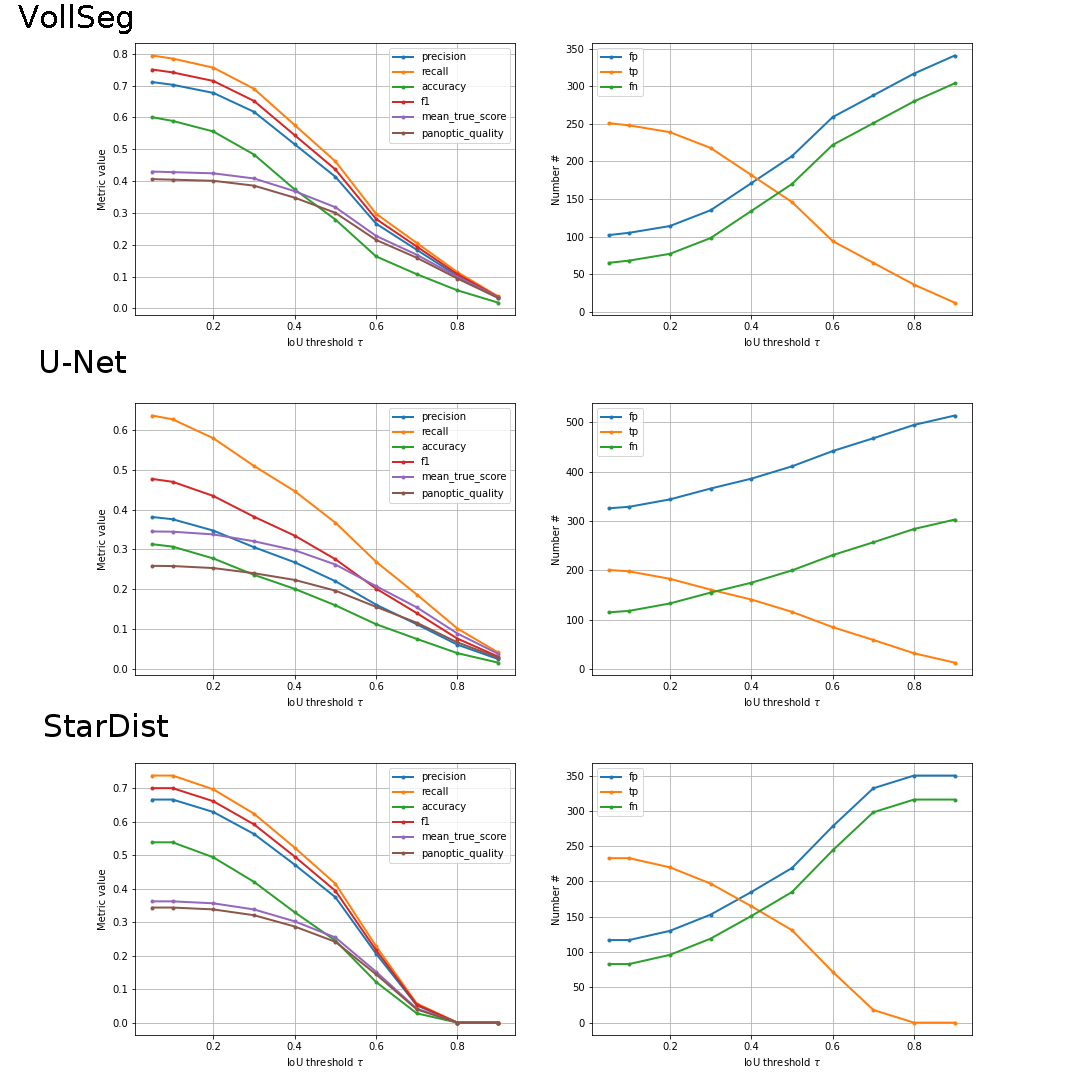
\includegraphics[width=\columnwidth]{figs/Metrics.png}}
\caption{Metric of comparision between 1) VollSeg, 2) Stardist, 3) Unet.}
\end{figure}\begin{figure}[]
\phantomsection\label{fig-mse}\noindent\makebox[\columnwidth][c]{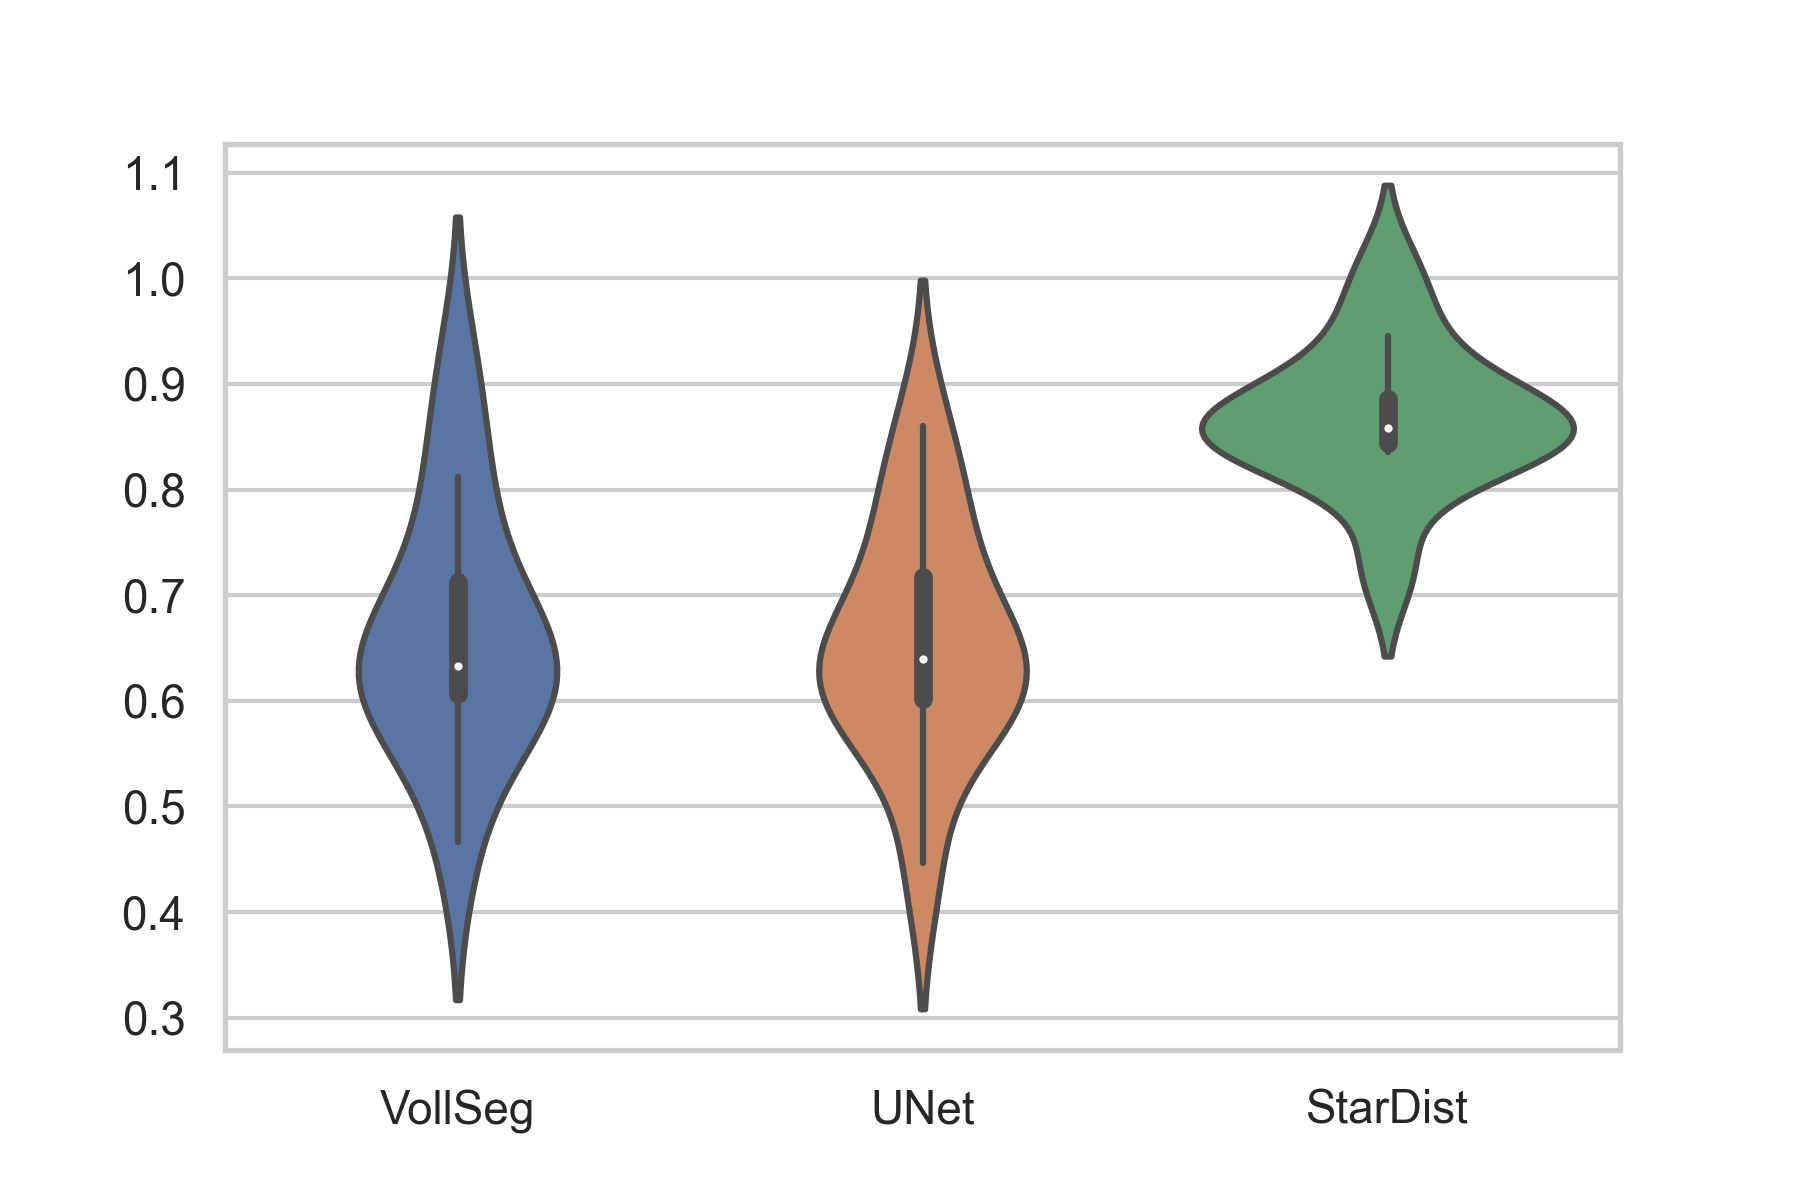
\includegraphics[width=\columnwidth]{figs/MSE.png}}
\caption{Mean Squared error comparision between VollSeg,  Stardist, Unet.}
\end{figure}\begin{figure}[]
\phantomsection\label{fig-gtvoll}\noindent\makebox[\columnwidth][c]{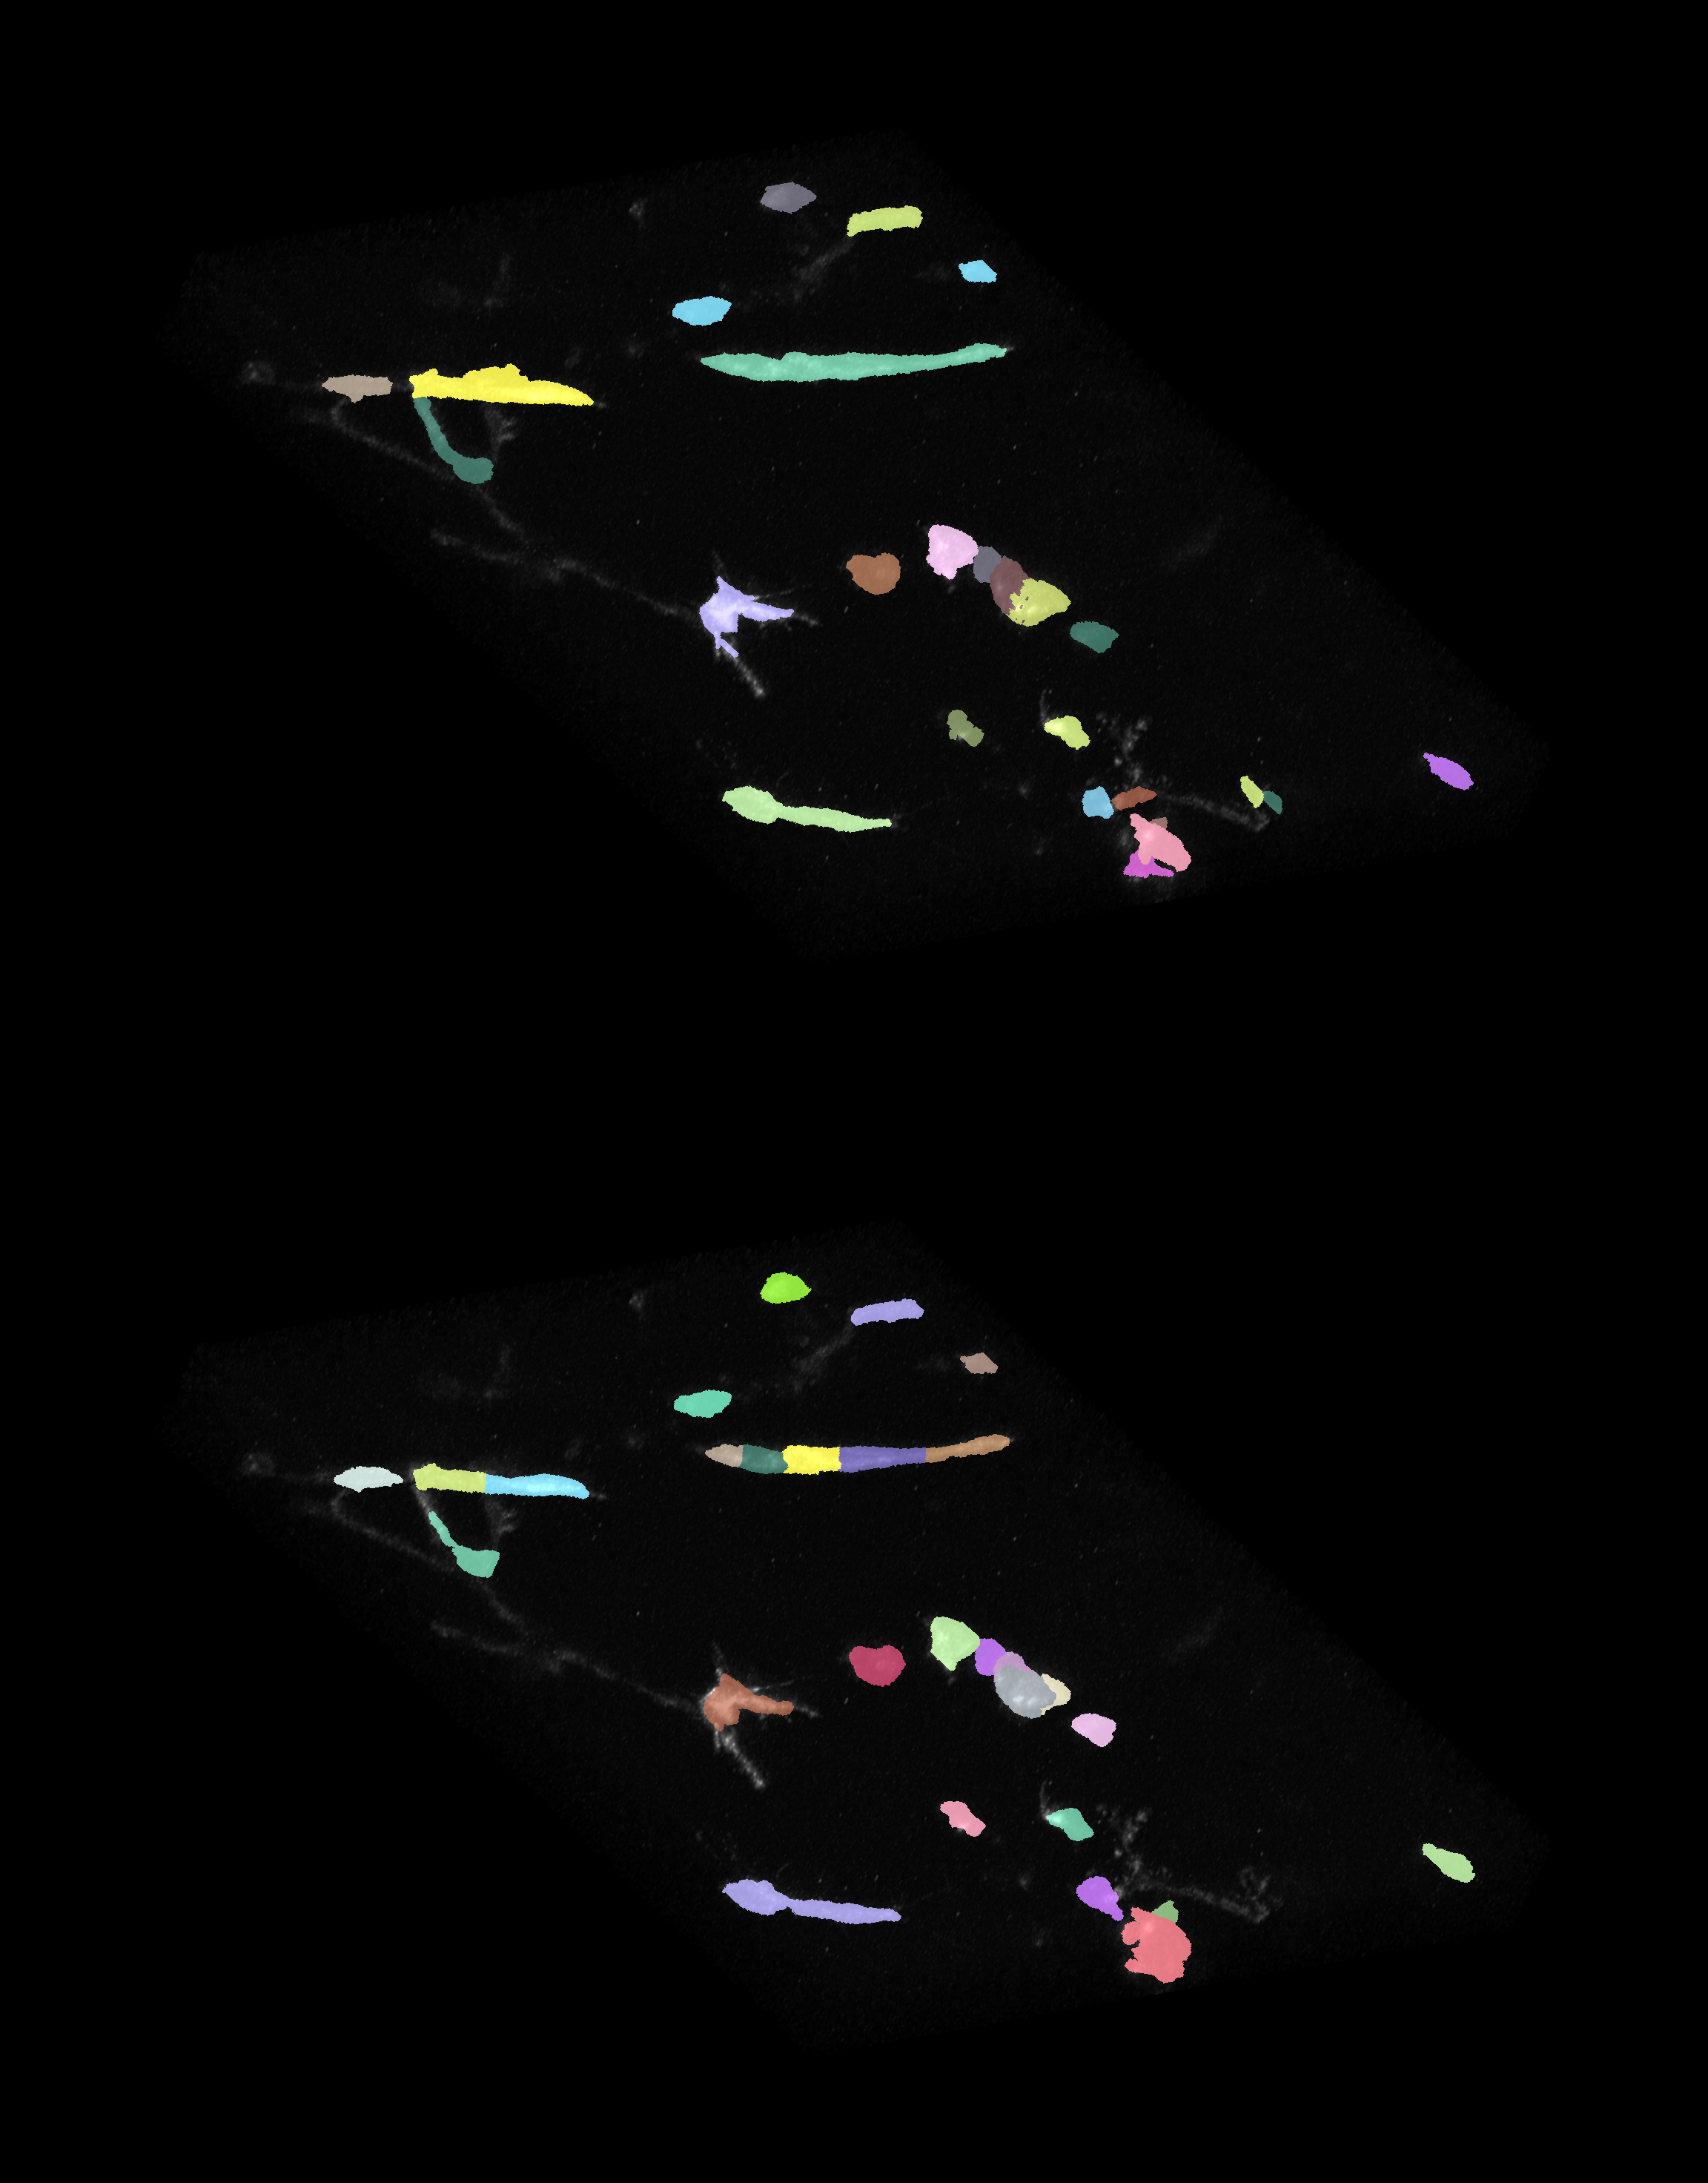
\includegraphics[width=\columnwidth]{figs/GTVoll.png}}
\caption{Visual 3D segmentation comparision between 1) GT segmentation (top) and 2) VollSeg segmentation (bottom).}
\end{figure}\begin{figure}[]
\phantomsection\label{fig-gtunet}\noindent\makebox[\columnwidth][c]{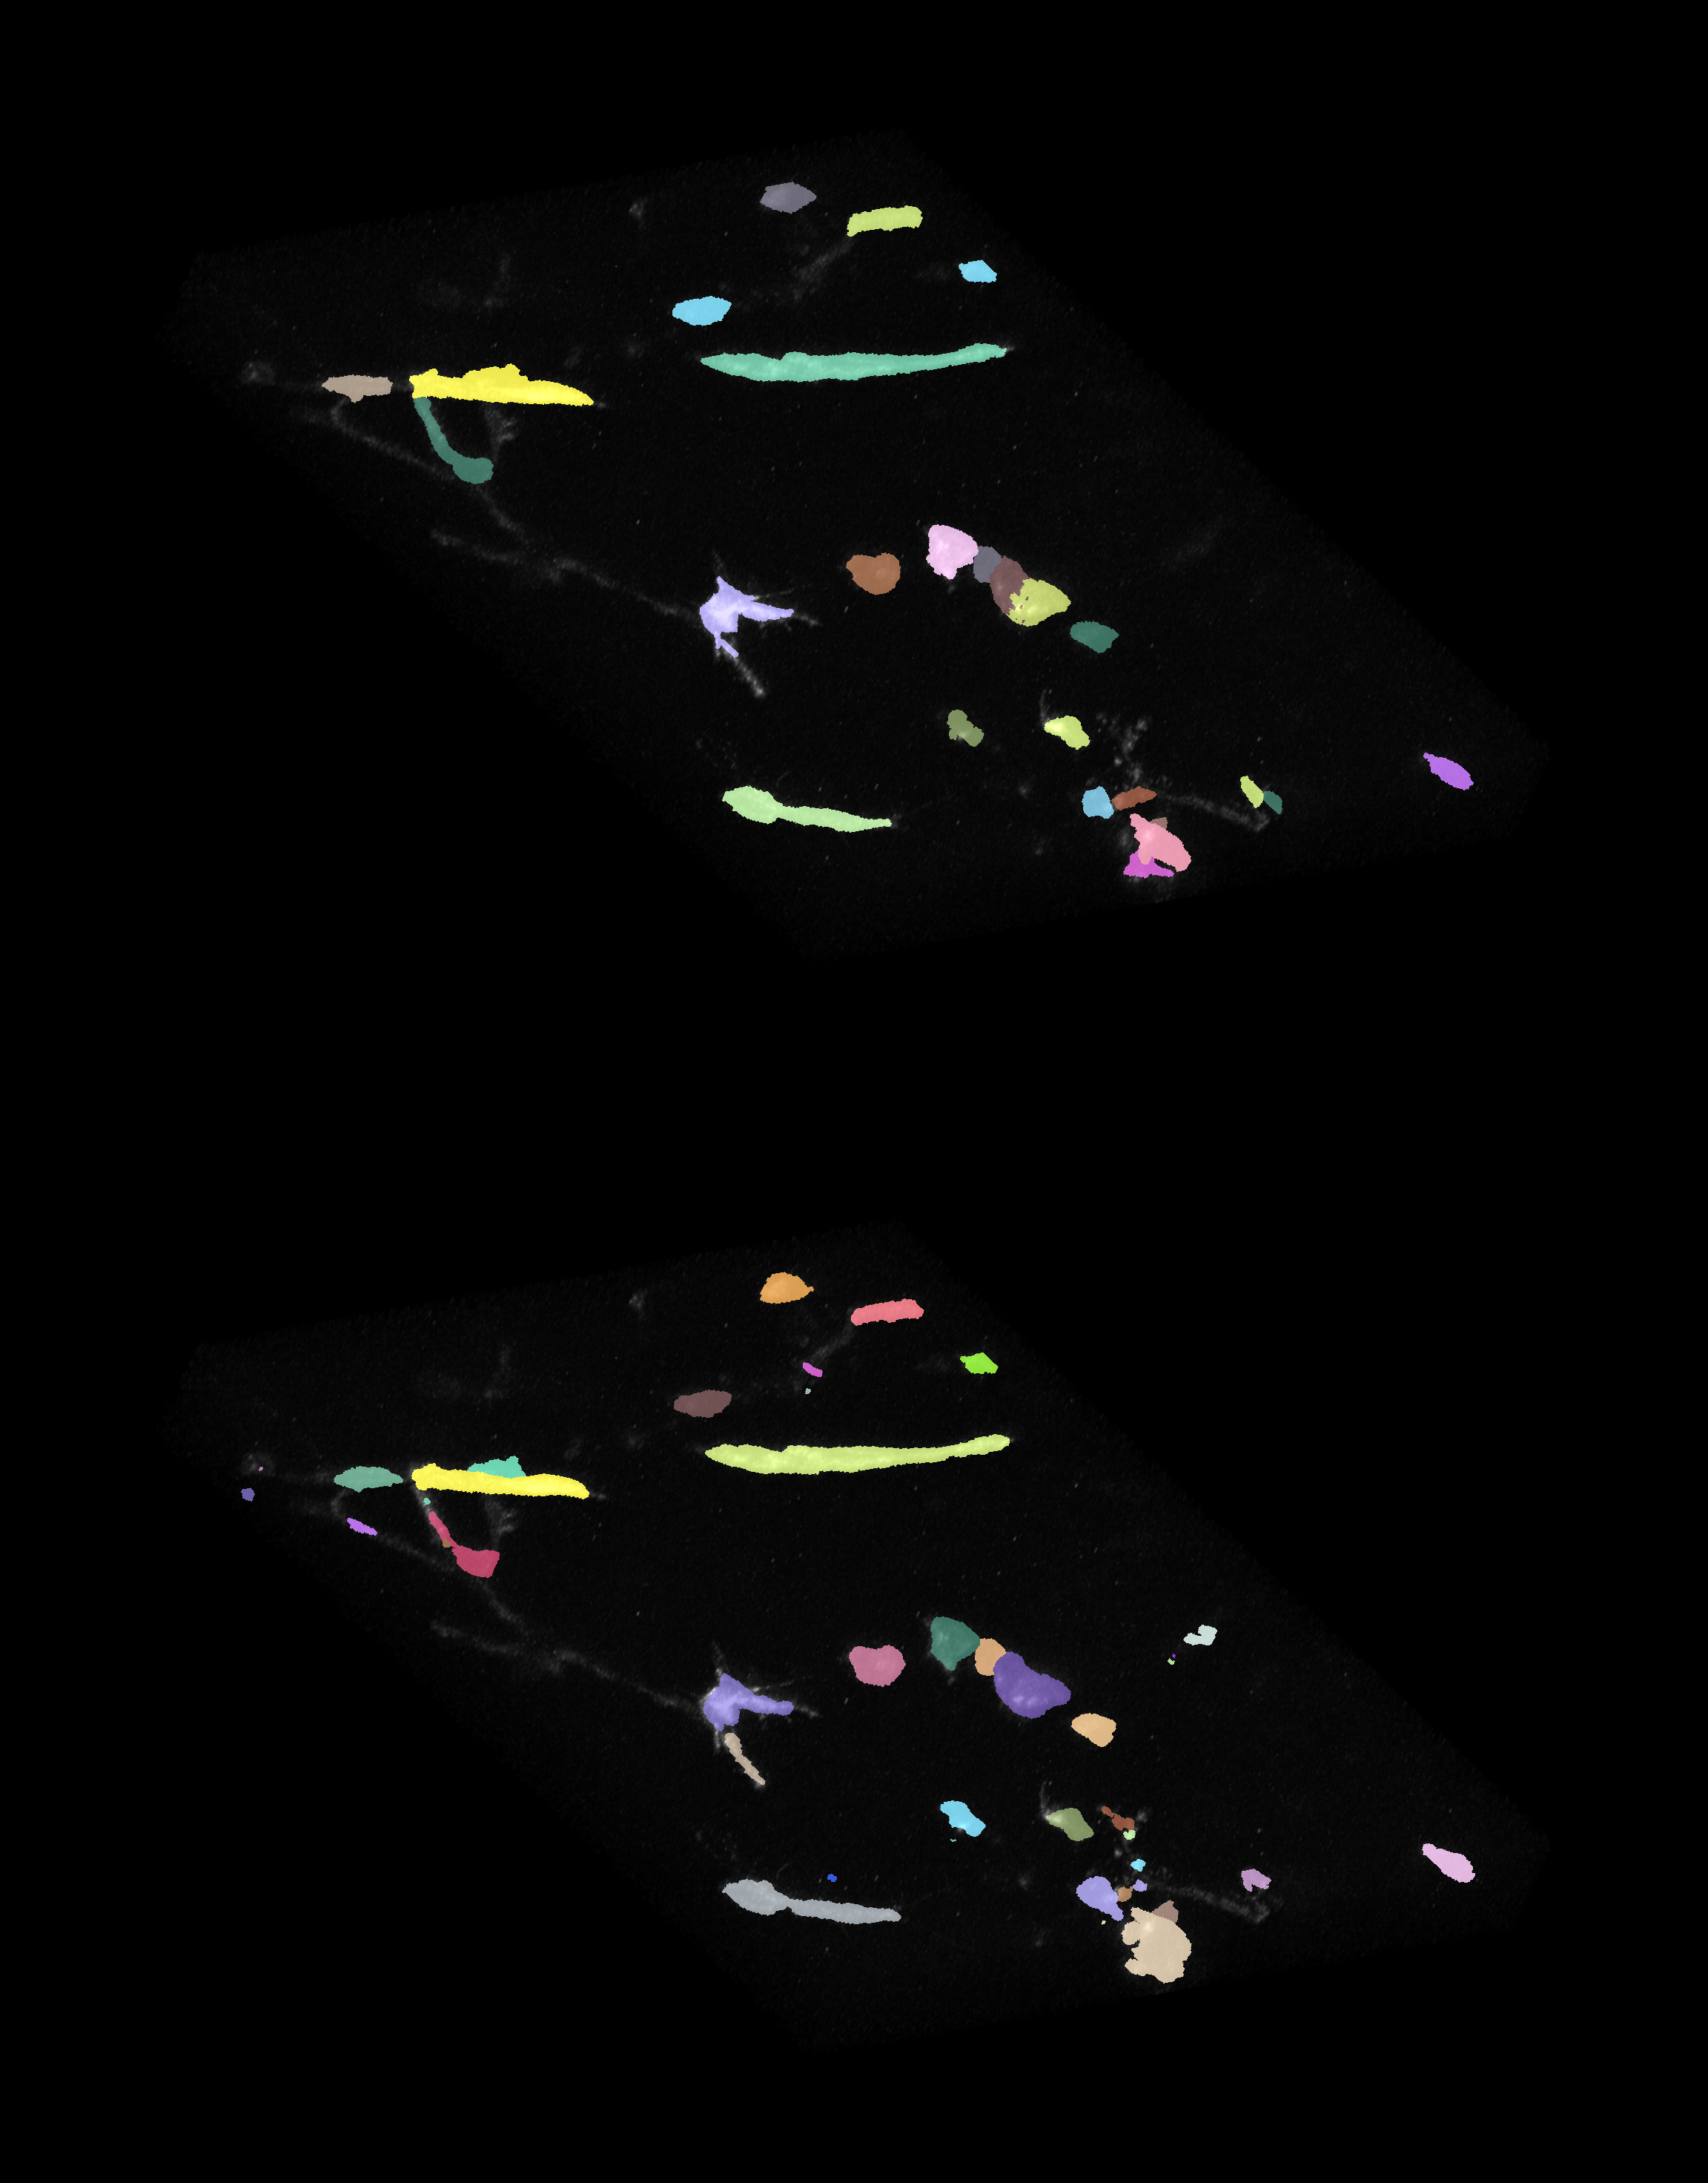
\includegraphics[width=\columnwidth]{figs/GTUnet}}
\caption{Visual  3D segmentation comparision between 1) GT segmentation (top) and 2) Unet segmentation (bottom).}
\end{figure}\begin{figure}[]
\phantomsection\label{fig-gtstar}\noindent\makebox[\columnwidth][c]{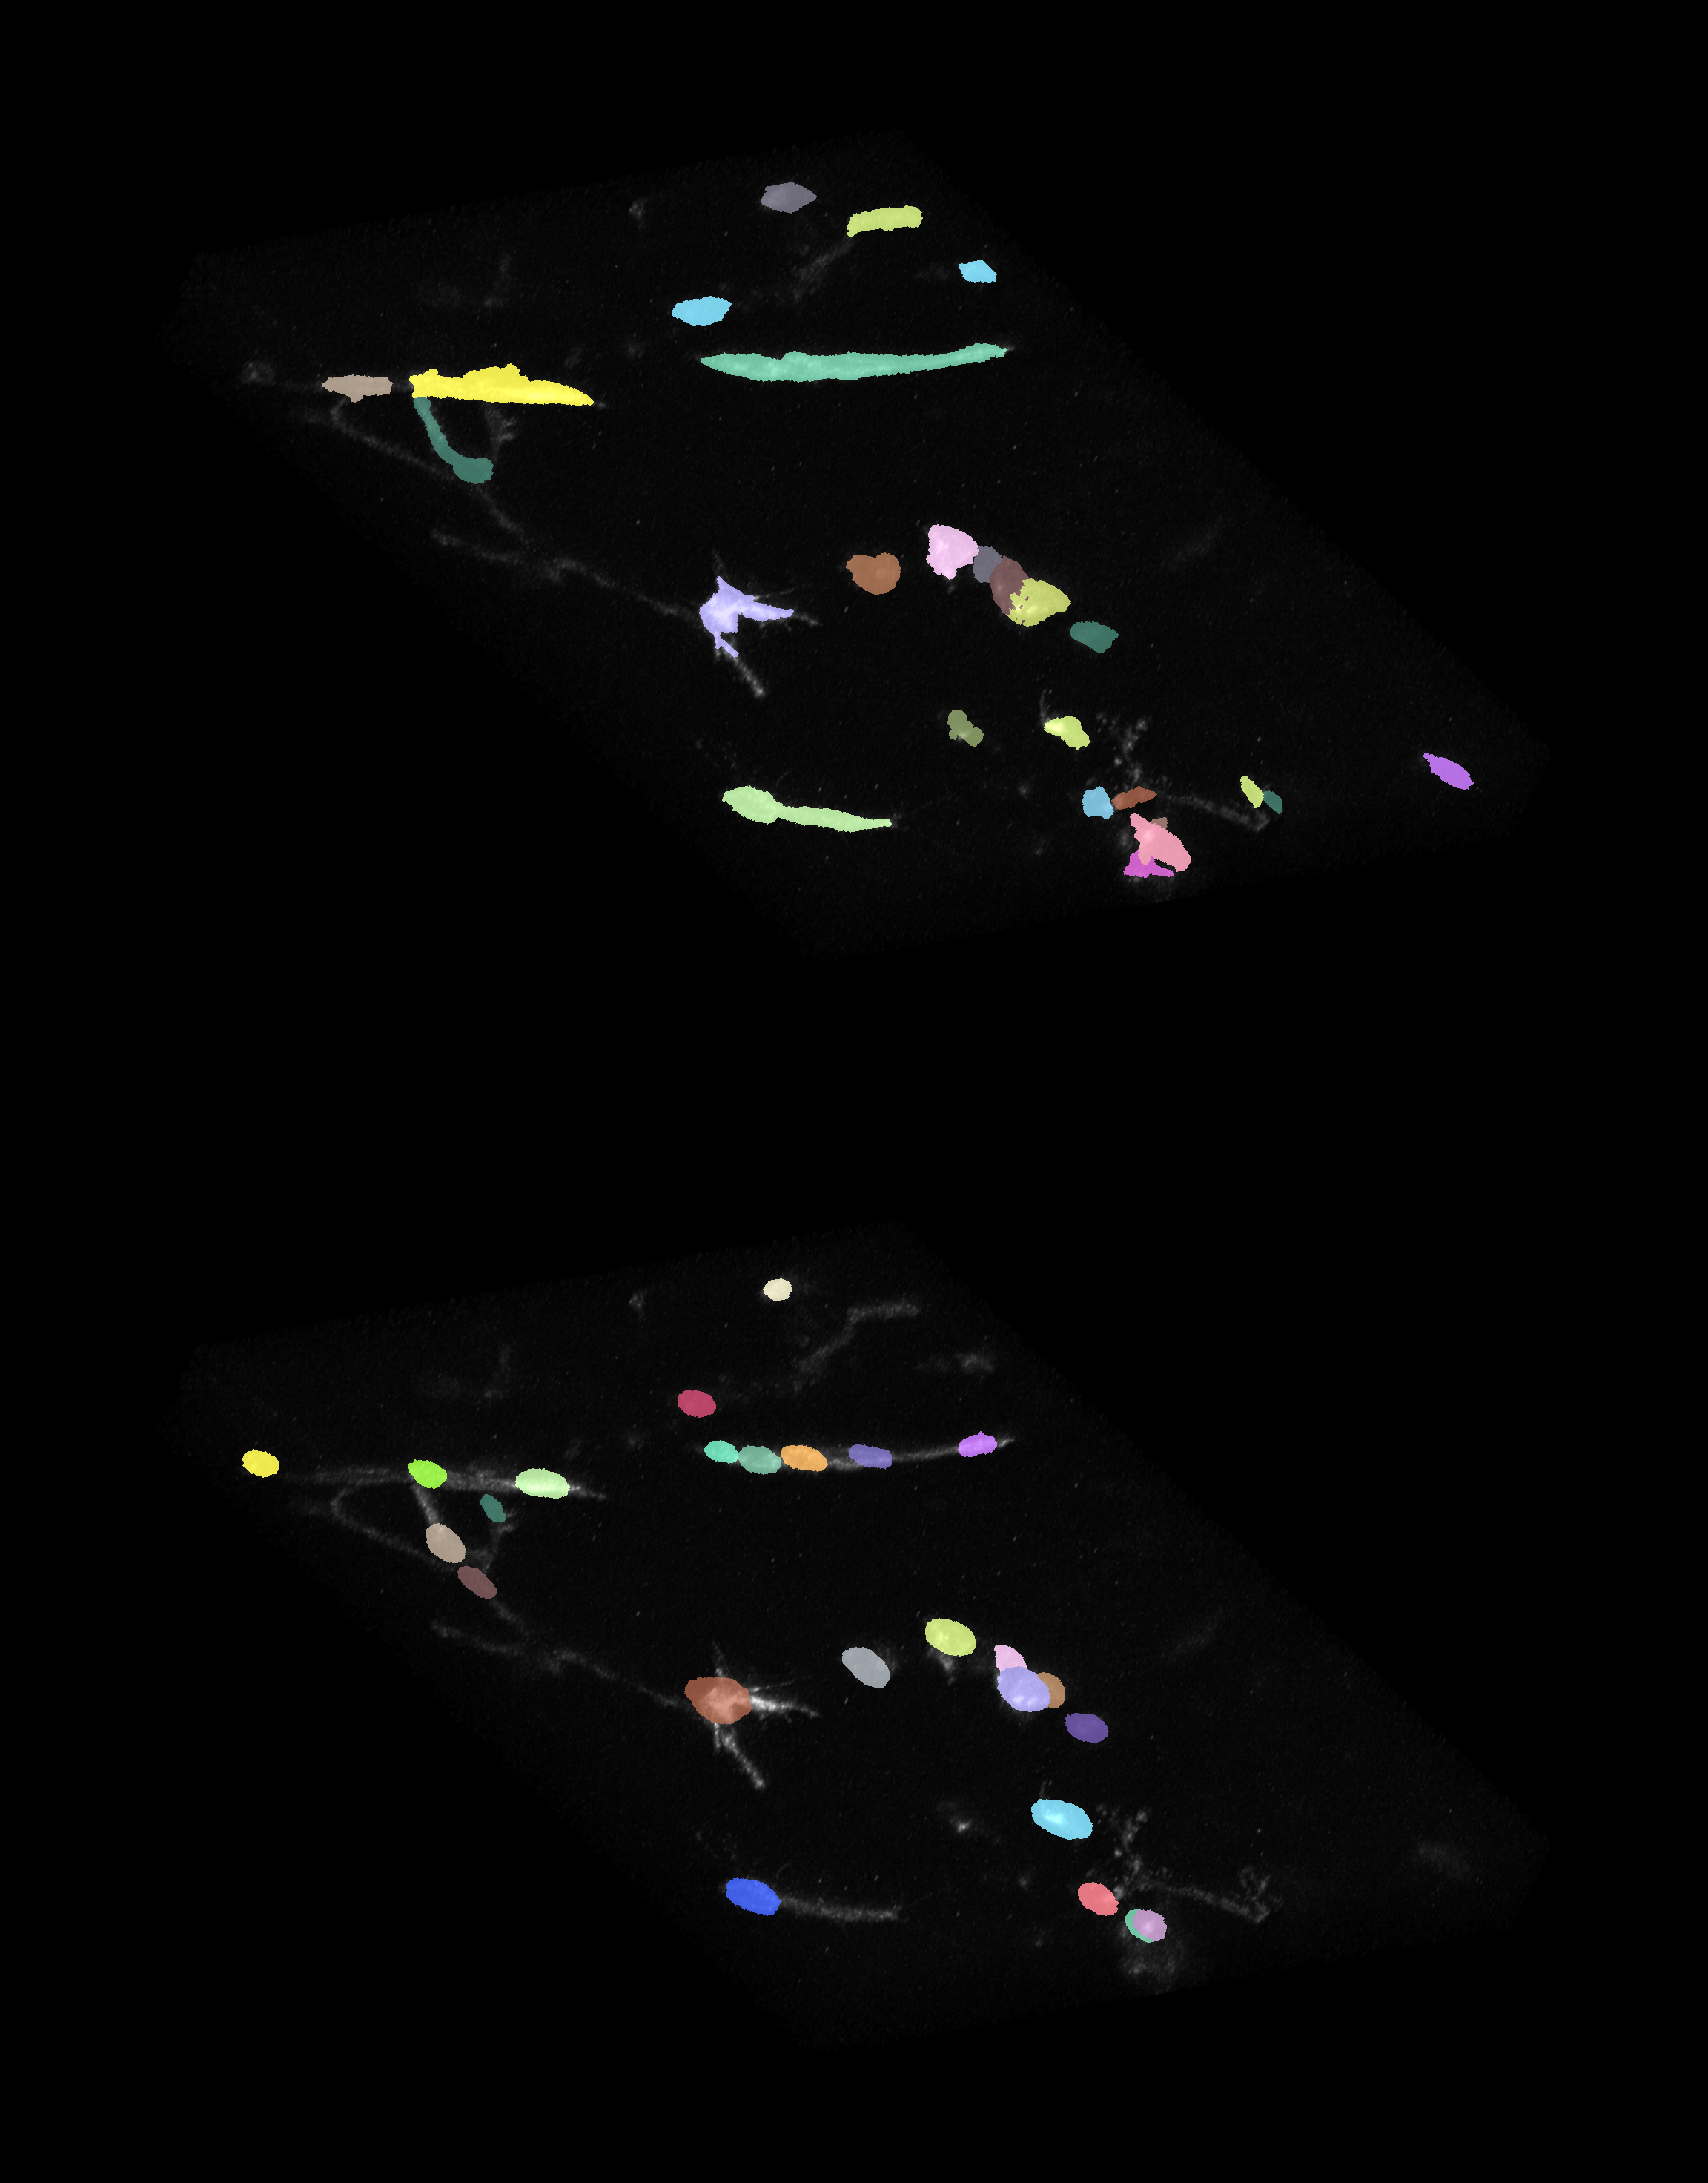
\includegraphics[width=\columnwidth]{figs/GTStar.png}}
\caption{Visual 3D segmentation comparision between 1) GT segmentation (top) and 2) Stardist segmentation (bottom).}
\end{figure}

The code for the seed criteria is shown below\vspace{1mm}
\begin{Verbatim}[commandchars=\\\{\},fontsize=\footnotesize]
\PY{k}{def} \PY{n+nf}{iou3D}\PY{p}{(}\PY{n}{boxA}\PY{p}{,} \PY{n}{centroid}\PY{p}{)}\PY{p}{:}

  \PY{n}{ndim} \PY{o}{=} \PY{n+nb}{len}\PY{p}{(}\PY{n}{centroid}\PY{p}{)}
  \PY{n}{inside} \PY{o}{=} \PY{k+kc}{False}

  \PY{n}{Condition} \PY{o}{=} \PY{p}{[}\PY{n}{Conditioncheck}\PY{p}{(}\PY{n}{centroid}\PY{p}{,} \PY{n}{boxA}\PY{p}{,} \PY{n}{p}\PY{p}{,} \PY{n}{ndim}\PY{p}{)}
   \PY{k}{for} \PY{n}{p} \PY{o+ow}{in} \PY{n+nb}{range}\PY{p}{(}\PY{l+m+mi}{0}\PY{p}{,}\PY{n}{ndim}\PY{p}{)}\PY{p}{]}

  \PY{n}{inside} \PY{o}{=} \PY{n+nb}{all}\PY{p}{(}\PY{n}{Condition}\PY{p}{)}

  \PY{k}{return} \PY{n}{inside}

\PY{k}{def} \PY{n+nf}{Conditioncheck}\PY{p}{(}\PY{n}{centroid}\PY{p}{,} \PY{n}{boxA}\PY{p}{,} \PY{n}{p}\PY{p}{,} \PY{n}{ndim}\PY{p}{)}\PY{p}{:}

    \PY{n}{condition} \PY{o}{=} \PY{k+kc}{False}

    \PY{k}{if} \PY{n}{centroid}\PY{p}{[}\PY{n}{p}\PY{p}{]} \PY{o}{\PYZgt{}}\PY{o}{=} \PY{n}{boxA}\PY{p}{[}\PY{n}{p}\PY{p}{]}
    \PY{o+ow}{and} \PY{n}{centroid}\PY{p}{[}\PY{n}{p}\PY{p}{]} \PY{o}{\PYZlt{}}\PY{o}{=} \PY{n}{boxA}\PY{p}{[}\PY{n}{p} \PY{o}{+} \PY{n}{ndim}\PY{p}{]}\PY{p}{:}

         \PY{n}{condition} \PY{o}{=} \PY{k+kc}{True}

    \PY{k}{return} \PY{n}{condition}
\end{Verbatim}
\vspace{1mm}
After obtaining the pool of seeds we can perform watershedding on either the distance map coming from stardist or the pixel probability map that is also an output of the stardist algorithm. We use U-net semantic segmentation as a mask in the watershedding process. The code for doing so is shown below\vspace{1mm}
\begin{Verbatim}[commandchars=\\\{\},fontsize=\footnotesize]
\PY{k}{def} \PY{n+nf}{WatershedwithMask3D}\PY{p}{(}\PY{n}{Image}\PY{p}{,} \PY{n}{Label}\PY{p}{,}\PY{n}{mask}\PY{p}{,} \PY{n}{grid}\PY{p}{)}\PY{p}{:}

  \PY{n}{properties} \PY{o}{=} \PY{n}{measure}\PY{o}{.}\PY{n}{regionprops}\PY{p}{(}\PY{n}{Label}\PY{p}{,} \PY{n}{Image}\PY{p}{)}
  \PY{n}{binaryproperties} \PY{o}{=}
  \PY{n}{measure}\PY{o}{.}\PY{n}{regionprops}\PY{p}{(}\PY{n}{label}\PY{p}{(}\PY{n}{mask}\PY{p}{)}\PY{p}{,} \PY{n}{Image}\PY{p}{)}
  \PY{n}{cord} \PY{o}{=}
  \PY{p}{[}\PY{n}{prop}\PY{o}{.}\PY{n}{centroid} \PY{k}{for} \PY{n}{prop} \PY{o+ow}{in} \PY{n}{properties}\PY{p}{]}
  \PY{n}{bin\PYZus{}cord} \PY{o}{=}
  \PY{p}{[}\PY{n}{prop}\PY{o}{.}\PY{n}{centroid} \PY{k}{for} \PY{n}{prop} \PY{o+ow}{in} \PY{n}{binaryproperties}\PY{p}{]}
  \PY{n}{Binarybbox} \PY{o}{=}
  \PY{p}{[}\PY{n}{prop}\PY{o}{.}\PY{n}{bbox} \PY{k}{for} \PY{n}{prop} \PY{o+ow}{in} \PY{n}{binaryproperties}\PY{p}{]}
  \PY{n}{cord} \PY{o}{=} \PY{n+nb}{sorted}\PY{p}{(}\PY{n}{cord} \PY{p}{,}
  \PY{n}{key}\PY{o}{=}\PY{k}{lambda} \PY{n}{k}\PY{p}{:} \PY{p}{[}\PY{n}{k}\PY{p}{[}\PY{l+m+mi}{0}\PY{p}{]}\PY{p}{,} \PY{n}{k}\PY{p}{[}\PY{l+m+mi}{1}\PY{p}{]}\PY{p}{,} \PY{n}{k}\PY{p}{[}\PY{l+m+mi}{2}\PY{p}{]}\PY{p}{]}\PY{p}{)}
  \PY{k}{if} \PY{n+nb}{len}\PY{p}{(}\PY{n}{Binarybbox}\PY{p}{)} \PY{o}{\PYZgt{}} \PY{l+m+mi}{0}\PY{p}{:}
          \PY{k}{for} \PY{n}{i} \PY{o+ow}{in} \PY{n+nb}{range}\PY{p}{(}\PY{l+m+mi}{0}\PY{p}{,} \PY{n+nb}{len}\PY{p}{(}\PY{n}{Binarybbox}\PY{p}{)}\PY{p}{)}\PY{p}{:}

              \PY{n}{box} \PY{o}{=} \PY{n}{Binarybbox}\PY{p}{[}\PY{n}{i}\PY{p}{]}
              \PY{n}{inside} \PY{o}{=}
              \PY{p}{[}\PY{n}{iou3D}\PY{p}{(}\PY{n}{box}\PY{p}{,} \PY{n}{star}\PY{p}{)} \PY{k}{for} \PY{n}{star} \PY{o+ow}{in} \PY{n}{cord}\PY{p}{]}

              \PY{k}{if} \PY{o+ow}{not} \PY{n+nb}{any}\PY{p}{(}\PY{n}{inside}\PY{p}{)} \PY{p}{:}
                       \PY{n}{cord}\PY{o}{.}\PY{n}{append}\PY{p}{(}\PY{n}{bin\PYZus{}cord}\PY{p}{[}\PY{n}{i}\PY{p}{]}\PY{p}{)}


  \PY{n}{cord}\PY{o}{.}\PY{n}{append}\PY{p}{(}\PY{p}{(}\PY{l+m+mi}{0}\PY{p}{,}\PY{l+m+mi}{0}\PY{p}{,}\PY{l+m+mi}{0}\PY{p}{)}\PY{p}{)}
  \PY{n}{cord} \PY{o}{=} \PY{n}{np}\PY{o}{.}\PY{n}{asarray}\PY{p}{(}\PY{n}{cord}\PY{p}{)}
  \PY{n}{cord\PYZus{}int} \PY{o}{=} \PY{n}{np}\PY{o}{.}\PY{n}{round}\PY{p}{(}\PY{n}{cord}\PY{p}{)}\PY{o}{.}\PY{n}{astype}\PY{p}{(}\PY{n+nb}{int}\PY{p}{)}

  \PY{n}{markers\PYZus{}raw} \PY{o}{=} \PY{n}{np}\PY{o}{.}\PY{n}{zeros\PYZus{}like}\PY{p}{(}\PY{n}{Image}\PY{p}{)}
  \PY{n}{markers\PYZus{}raw}\PY{p}{[}\PY{n+nb}{tuple}\PY{p}{(}\PY{n}{cord\PYZus{}int}\PY{o}{.}\PY{n}{T}\PY{p}{)}\PY{p}{]} \PY{o}{=}
  \PY{l+m+mi}{1} \PY{o}{+} \PY{n}{np}\PY{o}{.}\PY{n}{arange}\PY{p}{(}\PY{n+nb}{len}\PY{p}{(}\PY{n}{cord}\PY{p}{)}\PY{p}{)}
  \PY{n}{markers} \PY{o}{=}
  \PY{n}{morphology}\PY{o}{.}\PY{n}{dilation}\PY{p}{(}\PY{n}{markers\PYZus{}raw}\PY{p}{,}
  \PY{n}{morphology}\PY{o}{.}\PY{n}{ball}\PY{p}{(}\PY{l+m+mi}{2}\PY{p}{)}\PY{p}{)}

  \PY{n}{watershedImage} \PY{o}{=}
  \PY{n}{watershed}\PY{p}{(}\PY{o}{\PYZhy{}}\PY{n}{Image}\PY{p}{,} \PY{n}{markers}\PY{p}{,} \PY{n}{mask}\PY{p}{)}

  \PY{k}{return} \PY{n}{watershedImage}\PY{p}{,} \PY{n}{markers}
\end{Verbatim}
\vspace{1mm}
Here the Label comes from stardist prediction and mask comes from the U-net prediction.
The result of this approach is a 3D instance segmentation which we obtain for the luminal cells as shown in Fig.\{1\}. In the software package we provide training and prediction notebooks for training the base U-net and stardist networks on your own dataset. The package comes with jupyter notebooks for training and prediction on local GPU servers and also on Google Colab.

\subsection{Interactive codebase%
  \label{interactive-codebase}%
}


To train your networks using vollseg, install the code via pip install vollseg in your tensorflow enviornment with python > 3.7 and < 3.9. The first notebook needed is the one with takes the training dataset as input and creates npz file for U-net training, specify the path to your data that contains the folder of Raw and Segmentation images with the same name of images to create training pairs. Also to be specified is the name of the generated npz file along with the model directory to store the h5 files of the trained model and the model name.\vspace{1mm}
\begin{Verbatim}[commandchars=\\\{\},fontsize=\footnotesize]
\PY{n}{Data\PYZus{}dir} \PY{o}{=} \PY{l+s+s1}{\PYZsq{}}\PY{l+s+s1}{/data/}\PY{l+s+s1}{\PYZsq{}}
\PY{n}{NPZ\PYZus{}filename} \PY{o}{=} \PY{l+s+s1}{\PYZsq{}}\PY{l+s+s1}{VolumeSeg}\PY{l+s+s1}{\PYZsq{}}
\PY{n}{Model\PYZus{}dir} \PY{o}{=} \PY{l+s+s1}{\PYZsq{}}\PY{l+s+s1}{/data/}\PY{l+s+s1}{\PYZsq{}}
\PY{n}{Model\PYZus{}Name} \PY{o}{=} \PY{l+s+s1}{\PYZsq{}}\PY{l+s+s1}{VolumeSeg}\PY{l+s+s1}{\PYZsq{}}
\end{Verbatim}
\vspace{1mm}
In the next cell specify the model parameters, these parameters are the patch size chosen for training in XYZ for making overlapping patches for training, the number of patches to make the training data are also to be specified. The network depth is an important hyperparameter, more the network depth more are the number of parameters in the network and the image patch size has to be big enough so that when downsampling happens with increasing depth the size of the image in the inner most layer is still greater than 1. Start number of convolutional filters is another crucial hyperparameter controlling the network learning capacity. The number of filters are double at each layer of the network and depending on the size of the training dataset and of the GPU memory capacity this parameter can be tuned when doing hyperparameter optimization to obtain the best model for the given dataset. In this cell as a first step we generate the npz file for U-net training by setting the boolean GenerateNPZ to be true. Then in the next cell we can either train U-net and stardist network sequentially by setting TrainUNET and TrainSTAR booleans to be true or the users can split the training task between two GPUs by making a copy of the notebook and training one network per notebook. The other parameters to be chosen are the number of epochs for training, kernel size of the convolutional filter, the number of rays for stardist network to create a distance map along these directions. Additionally some of the OpenCL computations can be perfromed on a GPU using gputools library and if that is installed in the enviornment you can set use\_gpu\_opencl to be true.\vspace{1mm}
\begin{Verbatim}[commandchars=\\\{\},fontsize=\footnotesize]
\PY{c+c1}{\PYZsh{}Network training parameters}
\PY{n}{NetworkDepth} \PY{o}{=} \PY{l+m+mi}{5}
\PY{n}{Epochs} \PY{o}{=} \PY{l+m+mi}{100}
\PY{n}{LearningRate} \PY{o}{=} \PY{l+m+mf}{1.0E\PYZhy{}4}
\PY{n}{batch\PYZus{}size} \PY{o}{=} \PY{l+m+mi}{1}
\PY{n}{PatchX} \PY{o}{=} \PY{l+m+mi}{256}
\PY{n}{PatchY} \PY{o}{=} \PY{l+m+mi}{256}
\PY{n}{PatchZ} \PY{o}{=} \PY{l+m+mi}{64}
\PY{n}{Kernel} \PY{o}{=} \PY{l+m+mi}{3}
\PY{n}{n\PYZus{}patches\PYZus{}per\PYZus{}image} \PY{o}{=} \PY{l+m+mi}{16}
\PY{n}{Rays} \PY{o}{=} \PY{l+m+mi}{128}
\PY{n}{startfilter} \PY{o}{=} \PY{l+m+mi}{48}
\PY{n}{use\PYZus{}gpu\PYZus{}opencl} \PY{o}{=} \PY{k+kc}{True}
\PY{n}{GenerateNPZ} \PY{o}{=} \PY{k+kc}{True}
\PY{n}{TrainUNET} \PY{o}{=} \PY{k+kc}{False}
\PY{n}{TrainSTAR} \PY{o}{=} \PY{k+kc}{False}
\end{Verbatim}
\vspace{1mm}
After the network has been trained it will save the config files of the training configuration for both the networks along with the weight vector file as h5 files that will be used by the prediction notebook.

For running the network prediction on XYZ shape images use the prediction notebook either locally or on Colab. In this notebook you only have to specify the path to the image and the model directory. The only two parameters to be set here are the number of tiles (for creating image patches to fit in the GPU memory) and min\_size in pixel units to discard segmented objects below that size. Since we perform watershed on either the probability map or the distance map coming out of stardist the users can choose the former by setting UseProbability variable to true or by default we use the distance map.  The code below operates on a directory of XYZ shape images.\vspace{1mm}
\begin{Verbatim}[commandchars=\\\{\},fontsize=\footnotesize]
\PY{n}{ImageDir} \PY{o}{=} \PY{l+s+s1}{\PYZsq{}}\PY{l+s+s1}{data/tiffiles/}\PY{l+s+s1}{\PYZsq{}}
\PY{n}{Model\PYZus{}Dir} \PY{o}{=} \PY{l+s+s1}{\PYZsq{}}\PY{l+s+s1}{data/}\PY{l+s+s1}{\PYZsq{}}
\PY{n}{SaveDir} \PY{o}{=} \PY{n}{ImageDir} \PY{o}{+} \PY{l+s+s1}{\PYZsq{}}\PY{l+s+s1}{Results/}\PY{l+s+s1}{\PYZsq{}}
\PY{n}{UNETModelName} \PY{o}{=} \PY{l+s+s1}{\PYZsq{}}\PY{l+s+s1}{UNETVolumeSeg}\PY{l+s+s1}{\PYZsq{}}
\PY{n}{StarModelName} \PY{o}{=} \PY{l+s+s1}{\PYZsq{}}\PY{l+s+s1}{VolumeSeg}\PY{l+s+s1}{\PYZsq{}}

\PY{n}{UnetModel} \PY{o}{=} \PY{n}{CARE}\PY{p}{(}\PY{n}{config} \PY{o}{=} \PY{k+kc}{None}\PY{p}{,}
\PY{n}{name} \PY{o}{=} \PY{n}{UNETModelName}\PY{p}{,}
\PY{n}{basedir} \PY{o}{=} \PY{n}{Model\PYZus{}Dir}\PY{p}{)}
\PY{n}{StarModel} \PY{o}{=} \PY{n}{StarDist3D}\PY{p}{(}\PY{n}{config} \PY{o}{=} \PY{k+kc}{None}\PY{p}{,}
\PY{n}{name} \PY{o}{=} \PY{n}{StarModelName}\PY{p}{,}
\PY{n}{basedir} \PY{o}{=} \PY{n}{Model\PYZus{}Dir}\PY{p}{)}
\PY{n}{Raw\PYZus{}path} \PY{o}{=}
\PY{n}{os}\PY{o}{.}\PY{n}{path}\PY{o}{.}\PY{n}{join}\PY{p}{(}\PY{n}{ImageDir}\PY{p}{,} \PY{l+s+s1}{\PYZsq{}}\PY{l+s+s1}{*.tif}\PY{l+s+s1}{\PYZsq{}}\PY{p}{)}
\PY{n}{filesRaw} \PY{o}{=}
\PY{n}{glob}\PY{o}{.}\PY{n}{glob}\PY{p}{(}\PY{n}{Raw\PYZus{}path}\PY{p}{)}
\PY{n}{filesRaw}\PY{o}{.}\PY{n}{sort}
\PY{n}{min\PYZus{}size} \PY{o}{=} \PY{l+m+mi}{5}
\PY{n}{n\PYZus{}tiles} \PY{o}{=} \PY{p}{(}\PY{l+m+mi}{1}\PY{p}{,}\PY{l+m+mi}{1}\PY{p}{,}\PY{l+m+mi}{1}\PY{p}{)}
\PY{k}{for} \PY{n}{fname} \PY{o+ow}{in} \PY{n}{filesRaw}\PY{p}{:}

     \PY{n}{SmartSeedPrediction3D}\PY{p}{(}\PY{n}{ImageDir}\PY{p}{,}
     \PY{n}{SaveDir}\PY{p}{,} \PY{n}{fname}\PY{p}{,}
     \PY{n}{UnetModel}\PY{p}{,} \PY{n}{StarModel}\PY{p}{,}
     \PY{n}{min\PYZus{}size} \PY{o}{=} \PY{n}{min\PYZus{}size}\PY{p}{,}
     \PY{n}{n\PYZus{}tiles} \PY{o}{=} \PY{n}{n\PYZus{}tiles}\PY{p}{,}
     \PY{n}{UseProbability} \PY{o}{=} \PY{k+kc}{False}\PY{p}{)}
\end{Verbatim}
\vspace{1mm}


\subsection{Tracking%
  \label{tracking}%
}
After we obtain the segmentation using our approach we create a csv file fo the cell attributes that include their location, size and volume of the segmented cells. We use this csv file of the cell attributes as input to the tracker along with the Raw image. The Raw image is used to measure the intensity signal of the segmented cels while the segmentation is used to do the localization of the cells which we want to track. We do the tracking in Fiji, which is a popular software among the biologists. We developed our code over the existing tracking solution called Trackmate cite\{TM\}. Trackmate uses linear assingment  problem (LAP) algorithm to do linking of the cells and uses Jaqman linker for linking the segments for dividing and merging trajectories. We introduced a new parameter of minimum tracklet length to aid in the track editing tools also provided in the software. Hence by introducing a biological context of not having very short trajectories we reduce the track editing effort to correct for the linking mistakes made by the program. For testing our tracking program we used a freely available dataset from the cell tracking challenge of a developing C.elegans embryo. Using our software we can remove cells from tracking which do not fit certain criteria such as being too small (hence most likely a segmentation mistake) or being low in intensity or outside the region of interest such as when we want to track cells only inside a tissue. For this dataset we kept 12,000 cells and after filtering short tracks kept about 50 tracks with and without division events. The track information is saved as an XML file and can be re-opened to perform track editing from the last saved checkpoint. This is particularly useful when editing tracks coming from a huge dataset.

For this dataset the track scheme along with overlayed tracks in shown in Fig. The trackscheme is interactive as selecting a node in the trackscheme highlights the cell in Green and by selecting a cell in the image highlights its location in the trackscheme. Extensive manual for using the track editing is available on Fiji wiki.\begin{figure}[]
\phantomsection\label{fig-trackscheme}\noindent\makebox[\columnwidth][c]{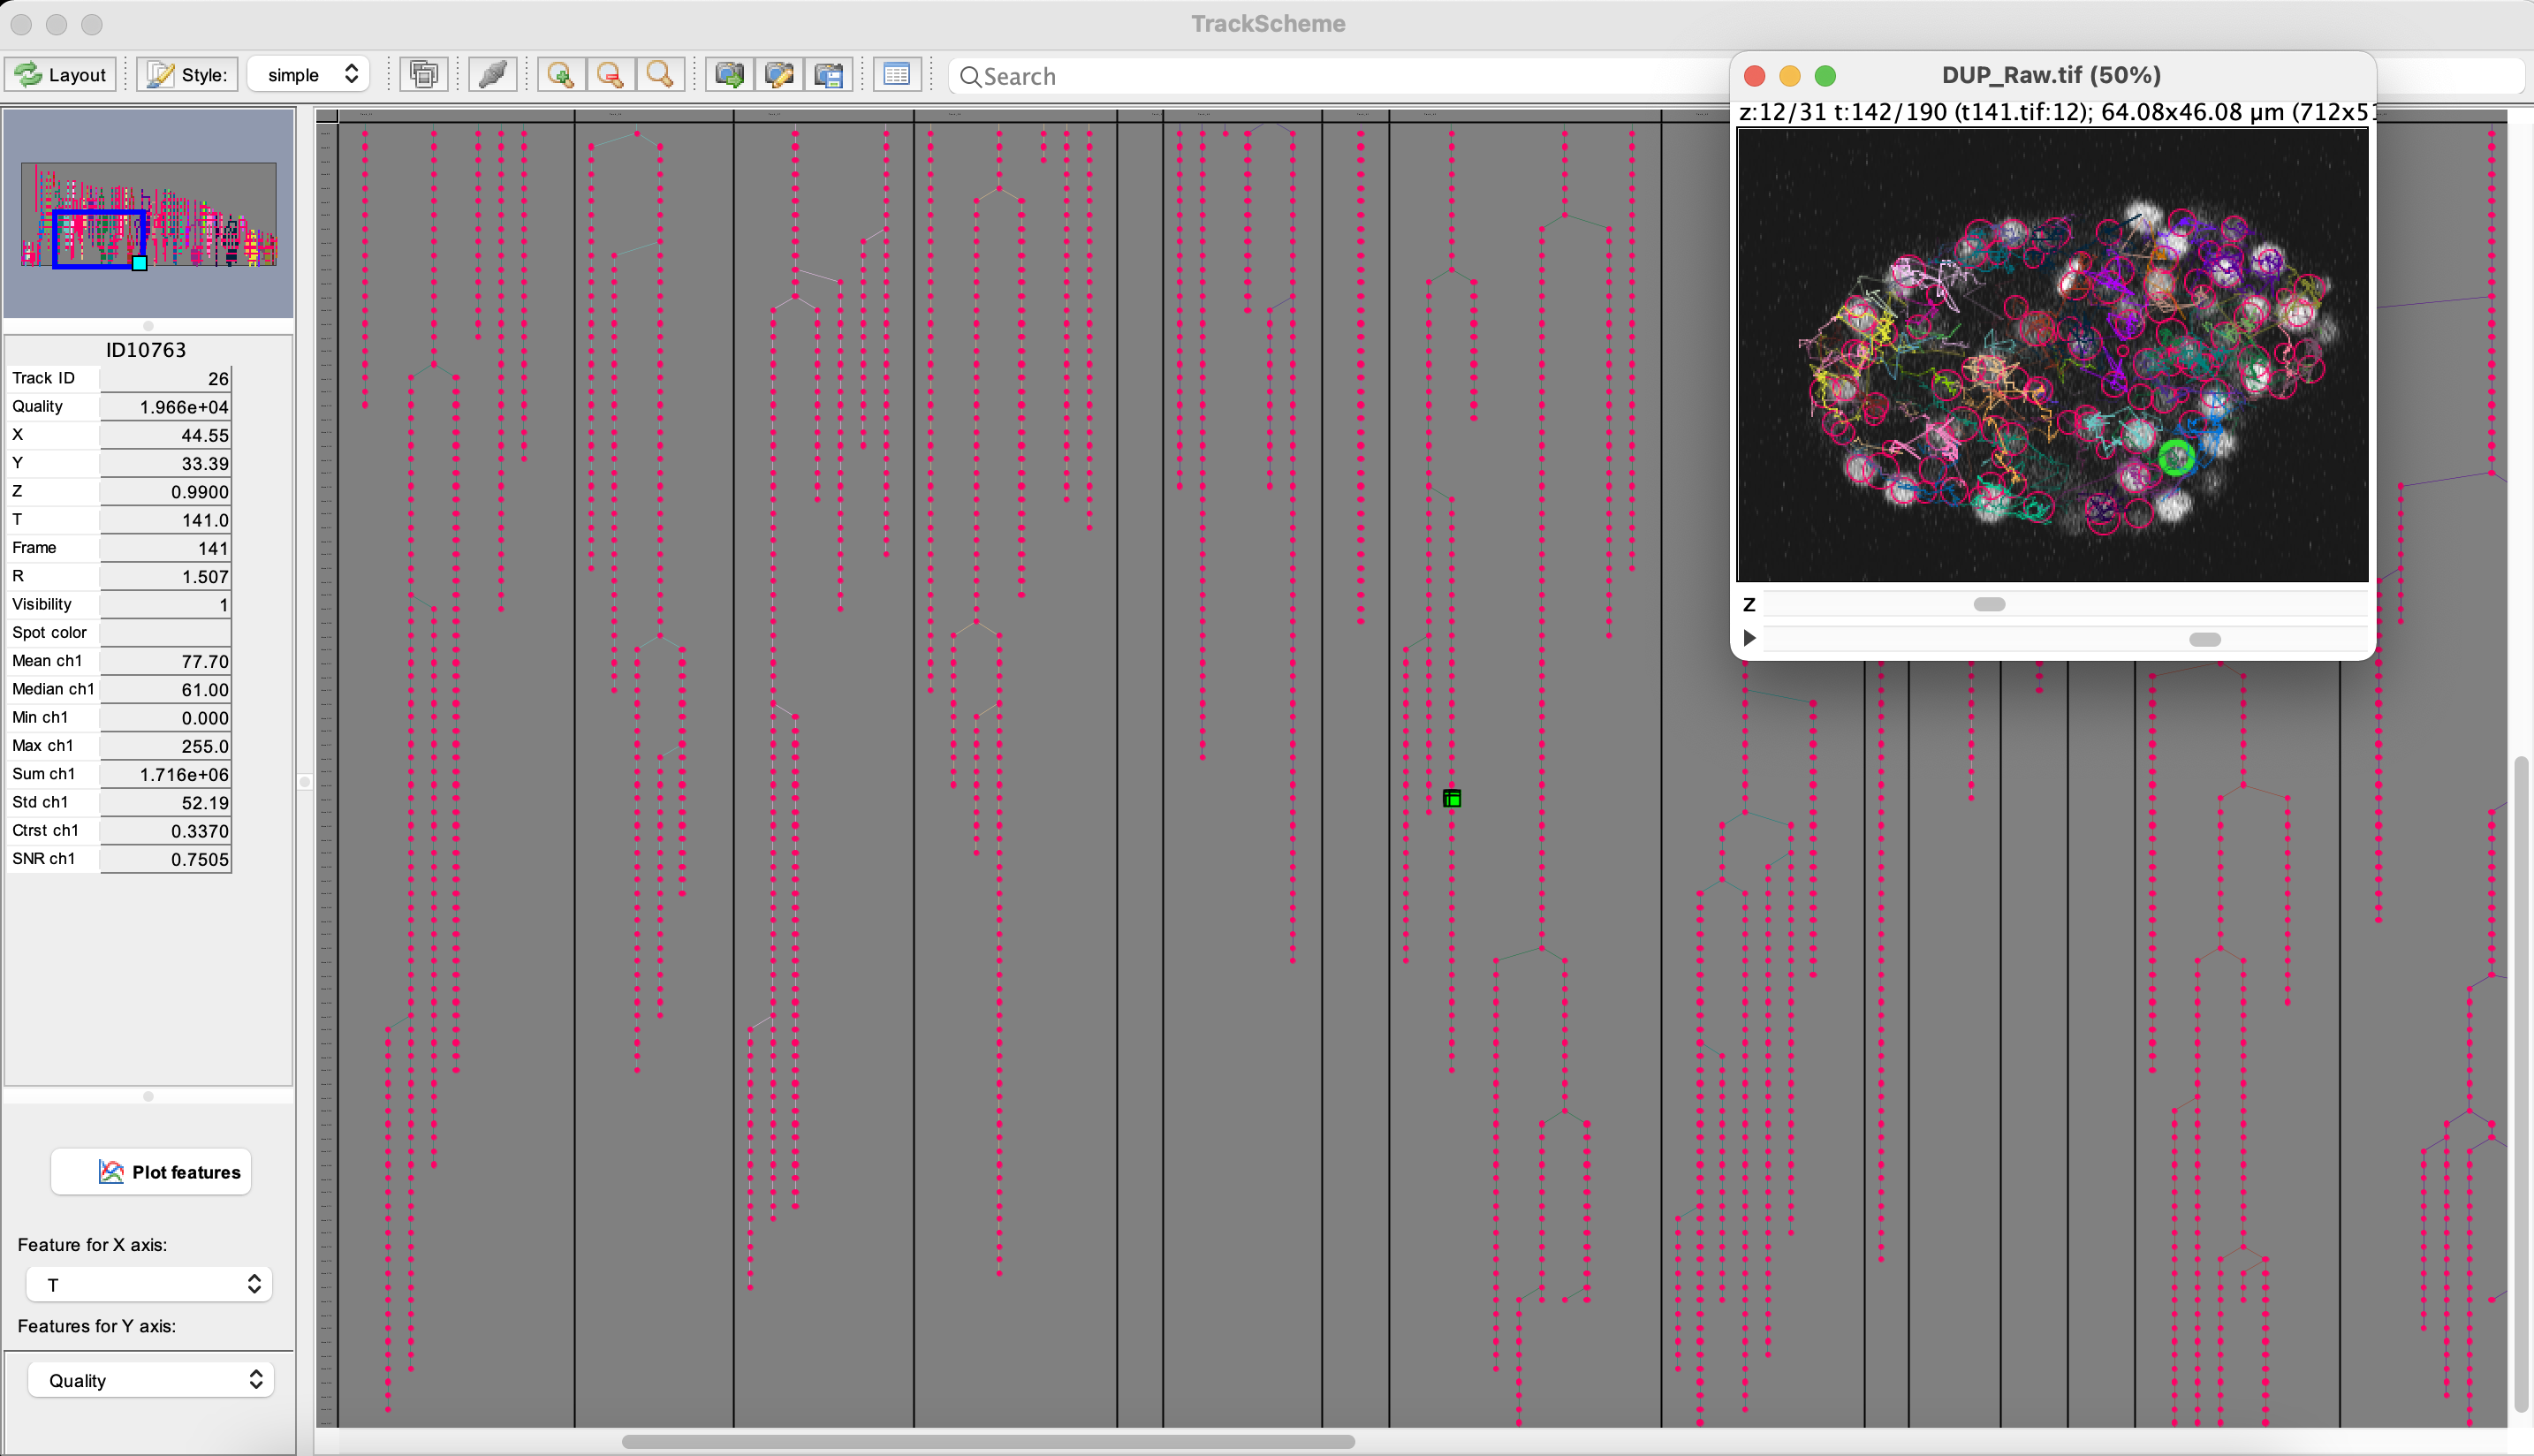
\includegraphics[width=\columnwidth]{figs/trackscheme.png}}
\caption{Trackscheme display for the C-elegans dataset.}
\end{figure}

\subsection{Track Analysis%
  \label{track-analysis}%
}


After obtaining the tracks from bTrackmate we save them as Trackmate XML file, this file contains the information about all the cells in a track. Since the cells can be highly erratic in their motions and move in not just the XY plane but also in Z we needed an Euler angle based viewer to view such tracks from different camera positions, recently a new and easy to use viewer based on python called Napari came into existence. Using this viewer we can easily navigate along multi dimensions, zoom and pan the view, toggle the visibility of image layers etc. We made a python package to bridge the gap between the Fiji and the Napari world by providing a track exporter that can read in the track XML files coming from the Fiji world and convert them into the tracks layer coming form the Fiji world. We use this viewer not just to view the tracks but also to analyze and extract the track information. As a first step we separate the dividing trajectories from the non-dividing trajectories, then in one notebook we compute the distance of the cells in the track from the tissue boundary and record the starting and the end distance of the root tracks and the succeeding tracklets of the daughter cells post division for dividing trajectories and only the root track for the non-dividing trajectory. This information is used to determine how cell chooses its fate, does it start from inside the tissue and remain inside during the duration of the experiment or does it move closer to the tissue boundary. This information is crucial when studying the organism in the early stage of development where the cells are highly dynamic and their fate is not known a priori.

Also another quantity of interest that can be obtained from the tools is quantification of intensity oscillations over time. In certain conditions there could be an intensity oscillation in the cells due to certain protein expression that leads to such oscillations, the biological question of interest is if such oscillations are stable and if so what is the period of the oscillation \DUrole{cite}{Ines}. Using our tool intensity of individual tracklet can be obtained which is then Fourier transformed to show the oscillation frequency if any. With this information we can see the contribution of each tracklet in the intensity oscillation and precisely associate the time when this oscillation began and ended.\begin{figure}[]
\phantomsection\label{fig-distancediv}\noindent\makebox[\columnwidth][c]{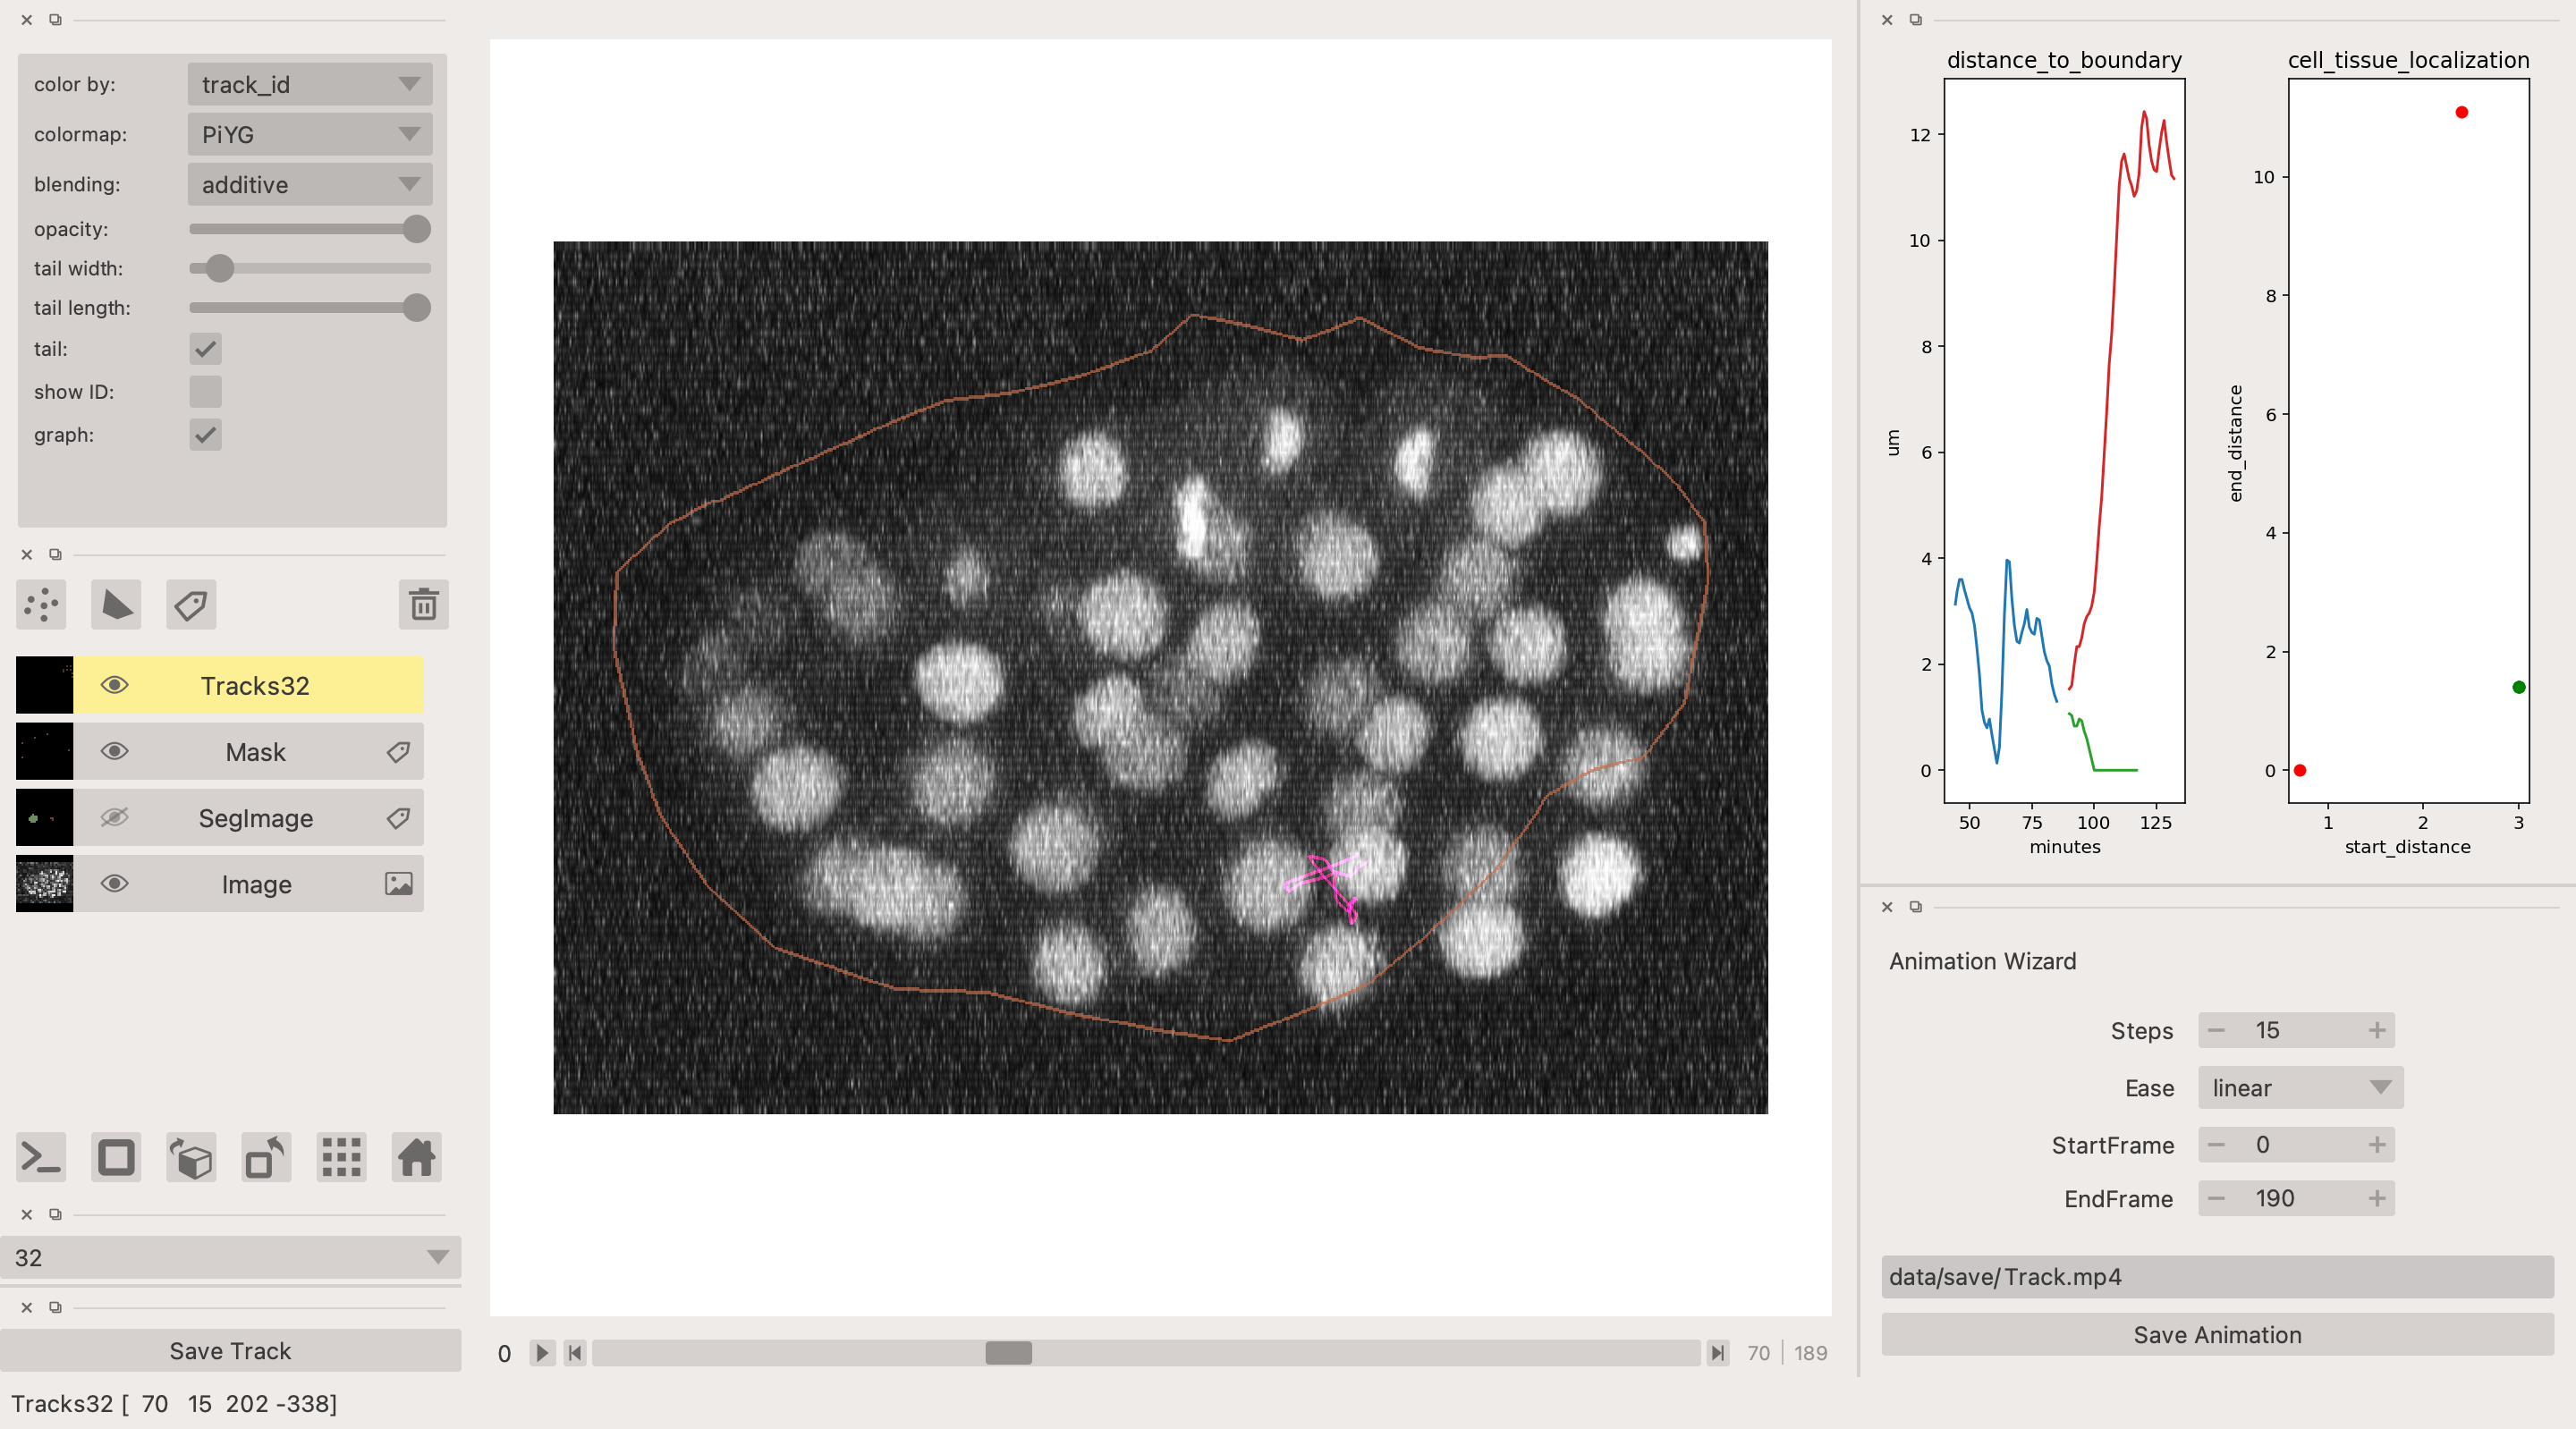
\includegraphics[width=\columnwidth]{figs/DistanceDividing1.png}}
\caption{Parent cell before division.}
\end{figure}\begin{figure}[]
\phantomsection\label{fig-distancediv2}\noindent\makebox[\columnwidth][c]{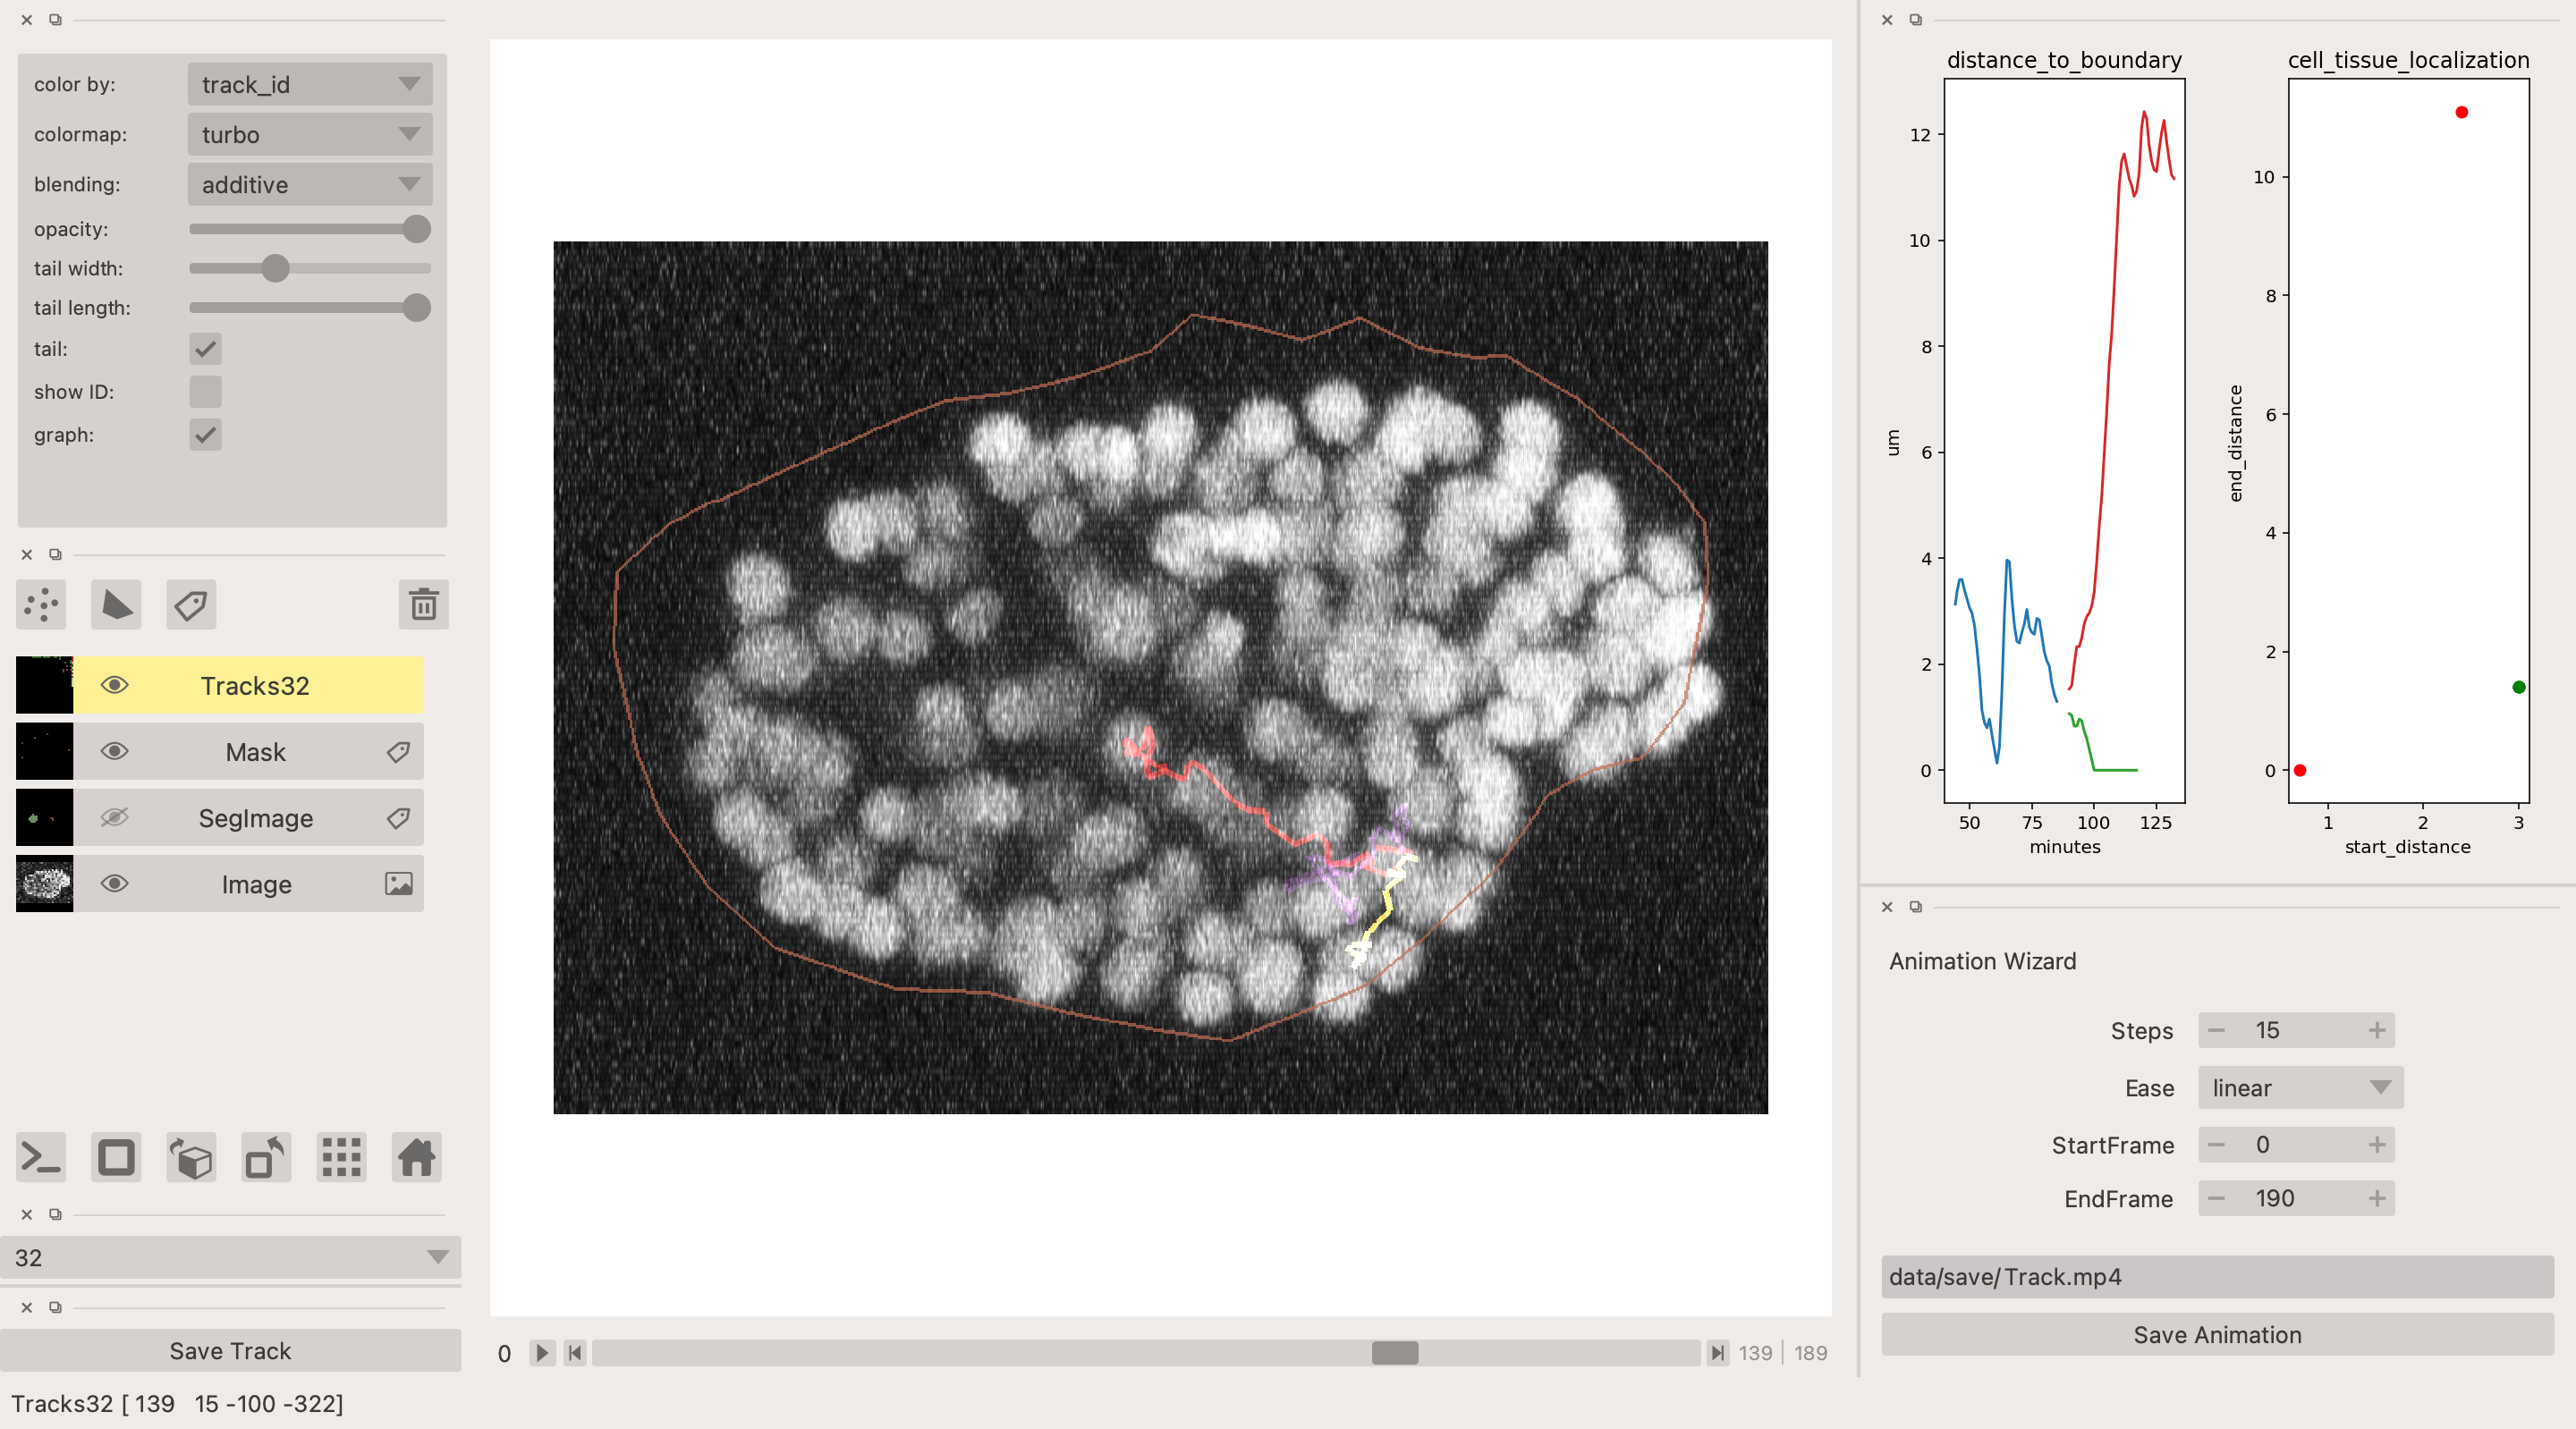
\includegraphics[width=\columnwidth]{figs/DistanceDividing2.png}}
\caption{Parent cell after division, one daughter cells moves inside while other stays close to the boundary.}
\end{figure}
\begin{thebibliography}{Stardist}
\bibitem[Stardist]{Stardist}{
\begin{enumerate}
\renewcommand{\labelenumi}{\Alph{enumi}.}
\setcounter{enumi}{20}
\item 

Schmidt, M. Weigert, C. Broaddus, and G. Myers,Cell detection with star-convex polygons, in Proceedings of MICCAI'18, 2018, pp. 265-273.\end{enumerate}
}
\bibitem[Unet]{Unet}{

Olaf Ronneberger, Philipp Fischer, and Thomas Brox, U-Net: Convolutional Networks for Biomedical Image Segmentation, in Proceedings of MICCAI'15, 2015, pp. 234-241.}
\bibitem[Ines]{Ines}{

Lahmann I, Brohl D, Zyrianova T, et al. Oscillations of MyoD and Hes1 proteins regulate the maintenance of activated muscle stem cells. Genes \& Development. 2019 May;33(9-10):524-535. DOI: 10.1101/gad.322818.118.}
\bibitem[TM]{TM}{

Tinevez JY, Perry N, Schindelin J, Hoopes GM, Reynolds GD, Laplantine E, Bednarek SY, Shorte SL, Eliceiri KW. TrackMate: An open and extensible platform for single-particle tracking. Methods. 2017 Feb 15;115:80-90. doi: 10.1016 j.ymeth.2016.09.016. Epub 2016 Oct 3. PMID: 27713081.}
\end{thebibliography}

\end{document}
